\RequirePackage{fix-cm}
\documentclass[10pt,journal,compsoc]{IEEEtran}

%\usepackage[toc,page]{appendix}
\usepackage{rotating}
\usepackage{subcaption}

\usepackage{cite}
\usepackage{graphicx}
\usepackage{multirow}
\usepackage{hhline}
\usepackage{comment}
\usepackage[dvipsnames]{xcolor}
\usepackage[colorlinks=false, linkcolor=blue, citecolor=blue, bookmarks=true,pagebackref=false]{hyperref}
\usepackage{hyphenat}
\usepackage{subcaption}
\usepackage{float}
\usepackage{caption}
\usepackage{fancybox}
\usepackage{array,booktabs}
\usepackage{marvosym} % For the \Letter command
%\usepackage{textcomp} % arrow
%\usepackage{tablefootnote} % footnote in table
\usepackage{balance}
\usepackage{ragged2e}
\usepackage{makecell}
\usepackage{bigstrut}
\newcolumntype{P}[1]{>{\centering\arraybackslash}p{#1}}
\usepackage{amssymb,mathtools}
\newcommand{\rqbox}[1]{
	\begin{center}
	\vspace{0cm}
	\cornersize{.2}
	\setlength{\fboxsep}{5pt}
	\ovalbox{\begin{minipage}{3.3in}
	{\em #1}
	\end{minipage}}
	\vspace{-0.1cm}

	\end{center}
}


\newcommand{\sw}[1]{\textcolor{red}{{\it [Shaowei says: #1]}}}
\newcommand{\jy}[1]{\textcolor{blue}{{\it [Jiayuan says: #1]}}}
\newcommand{\cp}[1]{\textcolor{red}{{\it [CP says: #1]}}}

\newcommand{\jyrm}[1]{\textcolor{blue}{{\it [REMOVE: #1]}}}

\newcommand{\code}[1]{{\texttt{#1}}}



\begin{document}

%=================== Title Here =================%
\title{Bounties in Open Source Development on GitHub: A Case Study of Bountysource Bounties}
%=================== Author Info Here =================%

\author{Jiayuan~Zhou,
        Shaowei~Wang,
        Cor-Paul~Bezemer,
        Ying~Zou,~\IEEEmembership{Member,~IEEE,}
        and~Ahmed~E.~Hassan,~\IEEEmembership{Member,~IEEE}
\IEEEcompsocitemizethanks{\IEEEcompsocthanksitem J. Zhou, S. Wang and A. E. Hassan are with the Software Analysis and Intelligence Lab (SAIL), Queen's University, Kingston, Ontario, Canada.\protect\\
% note need leading \protect in front of \\ to get a newline within \thanks as
% \\ is fragile and will error, could use \hfil\break instead.
E-mail: {jzhou,shaowei,ahmed}@cs.queensu.ca
\IEEEcompsocthanksitem CP Bezemer is with the Department of Electrical and Computer Engineering, University of Alberta, Edmonton,
              AB, Canada
E-mail: bezemer@ualberta.ca
\IEEEcompsocthanksitem Y. Zou is with the Department of Electrical and Computer Engineering, Queen's University, Kingston, Ontario, Canada.\protect\\
E-mail: ying.zou@queensu.ca
\IEEEcompsocthanksitem Shaowei Wang is the corresponding author.
}

}

% The paper headers
%\markboth{Journal of \LaTeX\ Class Files,~Vol.~14, No.~8, August~2015}%
%{Shell \MakeLowercase{\textit{et al.}}: Bare Demo of IEEEtran.cls for Computer Society Journals}

% in the abstract or keywords.
\IEEEtitleabstractindextext{

\begin{abstract}
Due to the voluntary nature of open source software, it can be hard to find a developer to work on a particular task. For example, some issue reports may be too cumbersome and unexciting for someone to volunteer to do them, yet these issue reports may be of high priority to the success of a project. To provide an incentive for implementing such issue reports, one can propose a monetary reward, i.e., a bounty, to the developer who completes that particular task.
In this paper, we study bounties in open source projects on GitHub to better understand how bounties can be leveraged to evolve such projects in terms of addressing issue reports.

We investigated 5,445 bounties for GitHub projects. These bounties were proposed through the Bountysource platform with a total bounty value of \$406,425.
We find that 1) in general, the timing of proposing bounties and the bounty-usage frequency are the most important factors that impact the likelihood of an issue being addressed. More specifically, issue reports are more likely to be addressed if they are for projects in which bounties are used more frequently and if they are proposed earlier. 2) The bounty value that an issue report has is the most important factor that impacts the issue-addressing likelihood in the projects in which no bounties were used before. Backers in such projects proposed higher bounty values to get issues addressed. 3) There is a risk of wasting money for backers who invest money on long-standing issue reports. 
%Based on our findings, we suggest that: 1) Backers should consider proposing a bounty as early as possible and are cautious when proposing bounties on long-standing issue reports. 2) Backers of projects with no former bounty-usage experience should consider proposing higher bounty values for issue reports.

\end{abstract}

% Note that keywords are not normally used for peerreview papers.
\begin{IEEEkeywords}
Software evolution, open source software, Bountysource, bounties, GitHub 
\end{IEEEkeywords}

}


%=================== Introduction Here =================%
% make the title area
\maketitle

%\IEEEdisplaynontitleabstractindextext

%\IEEEpeerreviewmaketitle

%\IEEEraisesectionheading{
\section{Introduction}\label{sec:introduction}
%Issue-fix is important

Software projects often use issue tracking systems to store and manage issue reports. Developers or users submit issue reports to report bugs or request new features, and wait for these issues to be addressed. However, some issue reports may never be addressed.
For example, developers may avoid addressing issues that they consider too low priority, or difficult to implement. To encourage developers to address such issue reports, a \textit{bounty} can be proposed by one or more \textit{backers} for the issue reports.

A bounty is a monetary reward that is often used in the area of software vulnerabilities. Prior studies examined the impact of bounties on vulnerability discovery \cite{zhao2017devising, hata2017understanding,finifter2013empirical}. Finifter et al.~\cite{finifter2013empirical} suggested that using bounties as an incentive to motivate developers to find security flaws is more cost-effective than hiring full-time security researchers.

Bounties are now being used to motivate developers to address issue reports, e.g., to fix bugs, to improve performance, or to add new features.
$Bountysource$\footnote{\url{https://www.bountysource.com}} is a platform for proposing bounties for open source projects across multiple platforms (e.g., GitHub) which currently has more than 46,000 registered developers.\footnote{\url{%https://blog.canya.com/2017/12/20/canya-acquires-majority-stake-in-bountysource-adds-over-46000-users/
http://bit.ly/2RkDeCc}} Although bounties are used in the issue-addressing process, the relationship between bounties and this process is not yet understood. For example, it is unclear whether a bounty improves the likelihood of an issue being addressed (i.e., the issue-addressing likelihood) in projects. By understanding this relationship, we could provide insights on how to better leverage bounties to evolve open source projects, and on how to improve the usability and effectivity of bounty platforms.


In this paper, we study 3,509 issue reports with 5,445 bounties that were proposed on Bountysource from 1,203 GitHub projects, with a total bounty value of \$406,425. We first examine the impact of the frequency of bounties (i.e., the bounty-usage frequency) being used in projects and the timing of proposing bounties on the likelihood of an issue being addressed. We found that:
\begin{enumerate}
    \item Bounty issue reports are more likely to be addressed in projects which are using bounties more frequently. Backers of the projects in which bounties were not used before proposed higher bounty values to get issues addressed.
    \item Bounty issue reports for which bounties were proposed earlier are more likely to be addressed. Additionally, there is a risk of wasting money for backers who invest money on long-standing issue reports.
\end{enumerate}

To understand if there are other factors that have an impact on the issue-addressing likelihood, we use logistic regression to study the relationship between 27 factors (including the timing of proposing a bounty and the bounty-usage frequency of a project) along 4 dimensions (i.e., project, issue, bounty, and backer) and the issue-addressing likelihood. We found that for bounty issue reports:
\begin{enumerate}
\item The timing of proposing bounties and the bounty-usage frequency are the two most important factors that impact the issue-addressing likelihood.
\item The total bounty value that an issue report has is the most important factor that impacts the issue-addressing likelihood in the first-timer projects.
\end{enumerate}


We also performed a manual study on the addressed bounty issue reports in which the bounty remained unclaimed (i.e., the cases in which bounties were ignored by developers). We found that some developers addressed an issue cooperatively, making it difficult to choose a single developer that would be awarded the bounty. In addition, some developers are not driven by money to address issues.

Based on our findings, we have several suggestions for backers and the Bountysource platform. For example, backers should be cautious when proposing small (i.e., $< \$100$) bounties on long-standing issue reports since the risk of losing the bounty exists. Bounty platforms should consider allowing for splittable multi-hunter bounties.



% the impact of the paper


The rest of the paper is organized as follows.
Section~\ref{background} presents background information about GitHub and Bountysource.
Section~\ref{dataset} describes our data collection process.
Section~\ref{prestudy} introduces our preliminary study.
Section~\ref{rq1} and Section~\ref{rq2} study the impact of the bounty on the issue-addressing likelihood in terms of projects' bounty-usage frequency and the timing of proposing bounties.
Section~\ref{rq3} investigates more factors that may potentially affect the issue-addressing likelihood.
 Section~\ref{sec:dis} studies the closed-unpaid bounty issue reports and discusses the implications of our study. Section~\ref{sec:threats} discusses the threats to validity of our study. Section~\ref{relatedwork} introduces related work. Finally, Section~\ref{conclusion} concludes our study.


%=================== Background =================%
\section{Background}
\label{background}
In this section, we briefly introduce the issue tracking system on GitHub and the open source bounty platform Bountysource.


\subsection{Issue tracking system on GitHub}

%\begin{figure*}[t]
%   \centering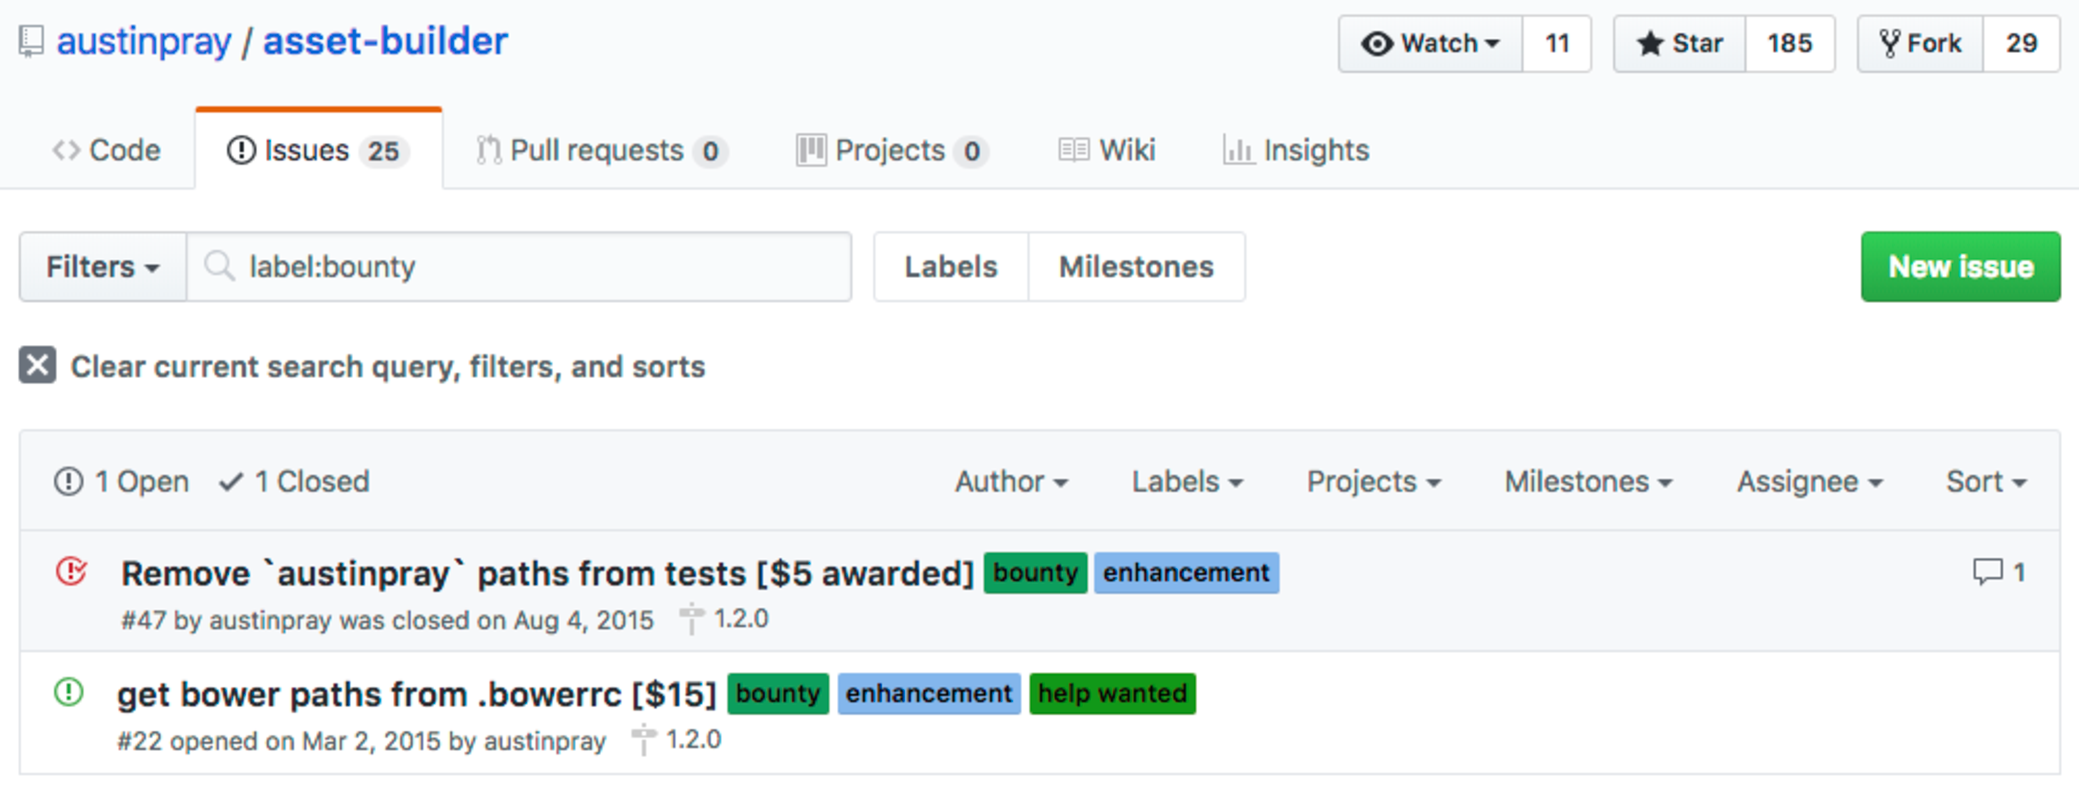
\includegraphics[width=17cm]{pics/bg/github_its}
%  \caption{Issue reports with a `bounty' label in the issue tracking system of the \code{austinpray/asset-builder} project on GitHub.}
%  \label{istdemo}
%\end{figure*}

The issue tracking system (i.e., ITS) on GitHub helps developers to manage the issue reports of their project. Users and developers can report bugs or request new features by posting an issue report on the issue tracking system. There are two statuses of an issue report: ``open'' and ``closed''. ``Open'' indicates that the issue report is still active and is waiting to be addressed. ``Closed'' indicates that the issue report has been closed. The most common reason for closing an issue report is that the issue has been addressed, but it could also have other reasons (e.g., duplicated issue reports).
Users can attach free-text labels to issue reports to indicate the category of an issue report.
An issue report contains a title to summarize the issue and a description that describes the issue in detail.
Developers can discuss an issue report by leaving comments, which can include code snippets, links or images to improve the description.
%For example, Figure~\ref{istdemo} lists two bounty issues\footnote{\url{https://github.com/austinpray/asset-builder/issues?q=label\%3Abounty}} of the \code{austinpray/asset-builder} project on GitHub. Both issues are tagged with the ``bounty'' label.



\subsection{Bountysource}
Bountysource is a platform on which users can pledge a monetary incentive (a \textit{bounty}) to address an issue report of an open source project.
There exist two roles on Bountysource: the bounty backer and the bounty hunter roles.

\noindent\textbf{Bounty backers}, which may be anonymous, are users or developers who propose bounties for issue reports. The backer can set an expiration period for bounties that are over \$100. When the bounty expires, the money is refunded to the backer; otherwise, the bounty stays with the issue report until someone claims it. Bounties that are smaller than \$100 are not refunded if they remain unclaimed. An issue report can have multiple bounties from one or more backers.

\noindent\textbf{Bounty hunters} are developers who address issue reports that have bounties. Once a developer claims to have addressed an issue report, its bounty backer(s) can choose to accept (no response will be taken as an acceptance) or reject the claim. In this situation, backers have two weeks to make the decision (accept or reject). If no backer explicitly rejects the claim, the bounties will be paid to the developer automatically.
Multiple bounty hunters can work on an issue report at the same time, but the bounties of an issue can only be rewarded to one bounty hunter.






Figure~\ref{RelationEntity} summarizes the relationships between the bounty, the bounty backer, the bounty hunter, the issue report, the issue reporter, and the developer. Basically, when an issue report is submitted by an issue reporter, one or more bounty backers can propose bounty(ies) on the issue report. One or more developers of the issue report can choose to become bounty hunters to address the issue report but only one bounty hunter can get the bounty(ies).




\begin{figure}[t]
   \centering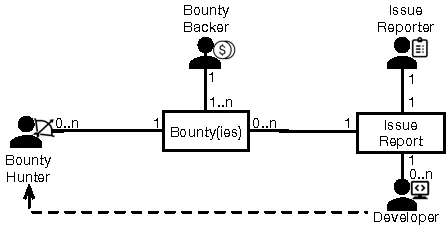
\includegraphics{pics/bg/RelationEntity}
      \vspace{-0.1in}
  \caption{The relationships between entities that are involved in the  bounty process.}
  \label{RelationEntity}
  \vspace{-0.1in}

\end{figure}

%There are two kinds of backer in Bountysource: 1) the personal backer, which represents an individual user. 2) The team backer, who represents a team or company (e.g., IBM).


Developers and users from more than 12 platforms (e.g., GitHub) propose bounties for issue reports through Bountysource. In this study, we focus on GitHub issue reports, since the majority of the bounties (see Section~\ref{dataset} for more details) that are proposed on Bountysource are for GitHub issue reports.
Figure~\ref{bountyflow} shows the workflow of the bounty processes between GitHub and Bountysource.
The lifecycle of a bounty starts with a bounty backer proposing a bounty for an issue report on GitHub. Bountysource will generate a link to the issue report on GitHub.
The bounty backers pledge money to Bountysource (the money is held by Bountysource) and can choose to ``advertise'' the bounty by tagging the issue report on GitHub with a bounty label (see the example\footnote{\url{%https://github.com/austinpray/asset-builder/issues?q=label\%3Abounty
http://bit.ly/2EQEA6c}} for details), appending the bounty value to the title of the issue report or mentioning the bounty in the discussion of the issue report in GitHub.
When a bounty hunter starts working on an issue, they can update their working status on Bountysource.
After the issue report is addressed, the bounty hunter can submit a claim for the bounty on Bountysource and the backer will be notified.
Once the bounty backer accepts the claim, the bounty hunter receives the money from Bountysource.

\begin{figure}[t]
   \centering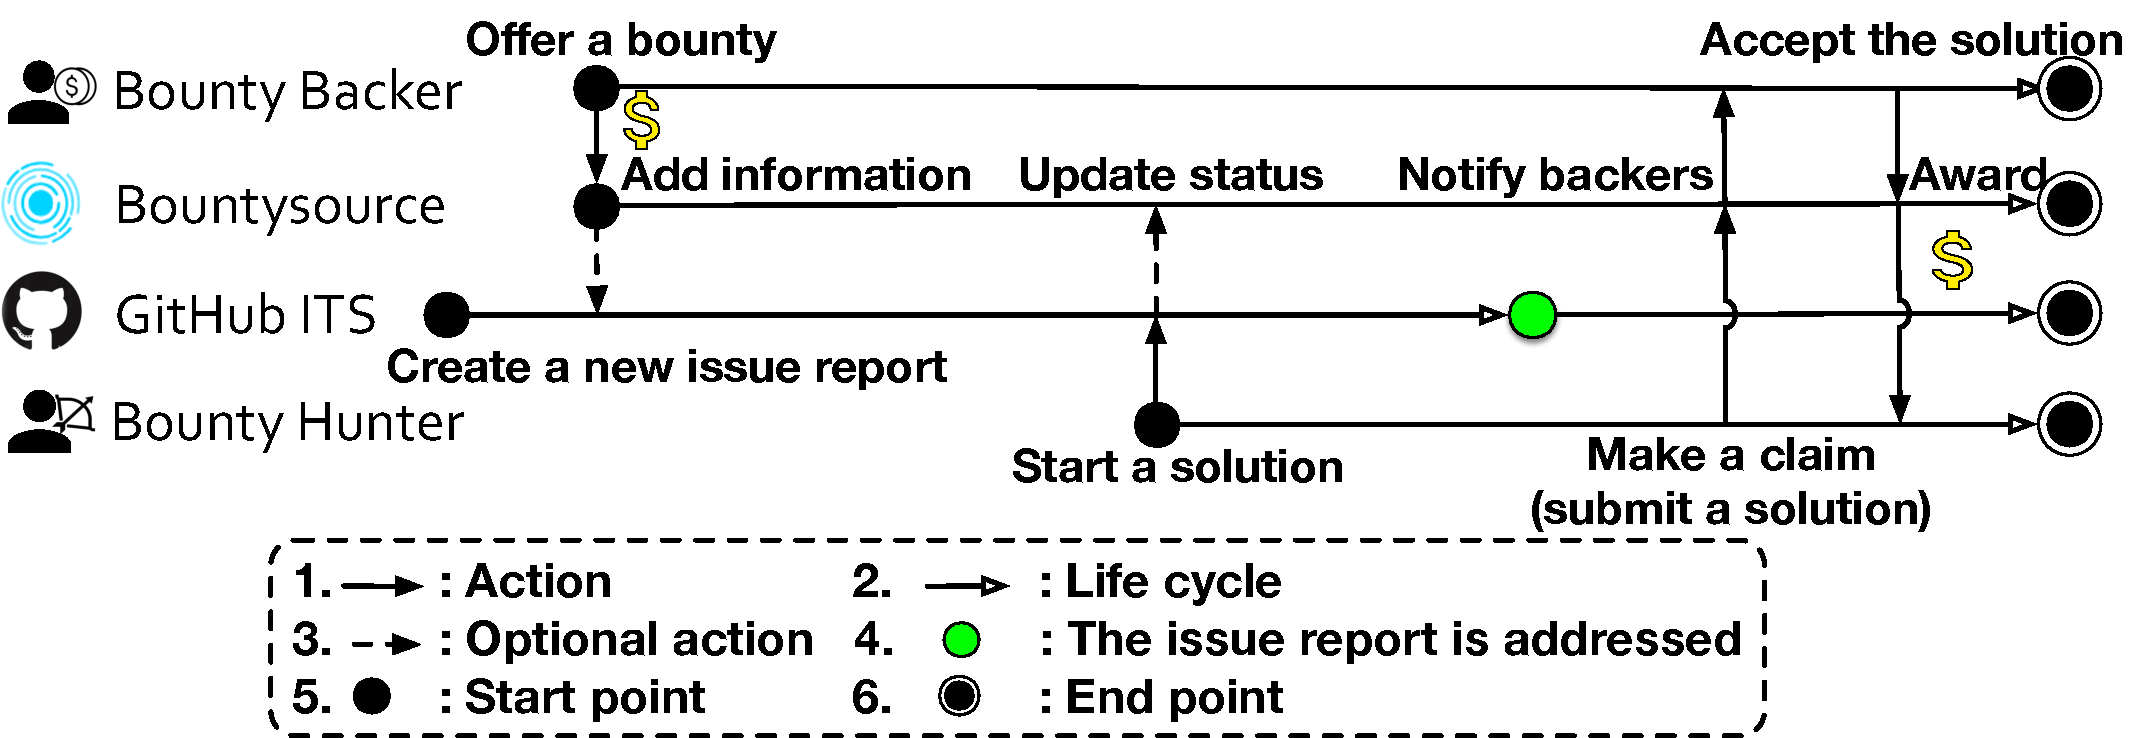
\includegraphics[width=9cm]{pics/bg/bountyflow}
   \vspace{-0.2in}
  \caption{The workflow of the bounty between GitHub and Bountysource.}
  \label{bountyflow}
  \vspace{-0.1in}

\end{figure}

Based on the status of an issue report and whether a bounty is paid out, a bounty issue report has the following three statuses:

\noindent\textbf{Closed-paid}: the issue report is closed and the bounty has been successfully rewarded to a bounty hunter. We defined such issue reports as \emph{successful} bounty issue reports.

\noindent\textbf{Open-unpaid}: the issue report is open and the bounty is active. We defined such issue reports as \emph{failed} bounty issue reports.

\noindent\textbf{Closed-unpaid}: the issue report is closed but the bounty remains unclaimed. We defined such issue reports as \emph{ignored} bounty issue reports.






%=================== Dataset Here =================%
\section{Data collection}
%\label{rq}
%
(RECONSTRUCT)In this section, we present our research questions and their motivation. In addition, we introduce the data collection approach to our study and present the basic statistics of the collected dataset at last. 
\subsection{Research Questions}

\textbf{RQ1: What is the impact of bounties in issue level?}\\
MOTIVATION AND BENEFIT
According to preliminary study, the bounty amount within different issues are quite different. Why the different is so big? Is a issue with higher bounty amount can get a higher possibility to be fixed? What is the bounty's impact in making a question fixing?
By studying the impact of bounties on issue-fixing, we can figure out how bounties affect issue-fixing process.



\noindent\textbf{RQ2: What is the impact of bounties in project level?}\\
What is the impact of bounty in project level? If a project decide to choose.

\noindent\textbf{RQ3: What causes the failure of bounties?}\\
MOTIVATION AND BENEFIT

\label{dataset}


In our study, we focus on the bounties that are proposed through the Bountysource platform since it is one of the most popular platforms for open source projects. As explained in Section~\ref{background}, Bountysource supports issue reports from several ITSs (e.g.,  GitHub and Bugzilla). Figure~\ref{RatioOfIssuesITS} shows the distribution of Bountysource bounties across its supported ITSs. The majority of the issue reports come from GitHub (77.3\%), hence we focus our study on the bounties that were proposed for GitHub issue reports.




\begin{figure}[t]
    \centering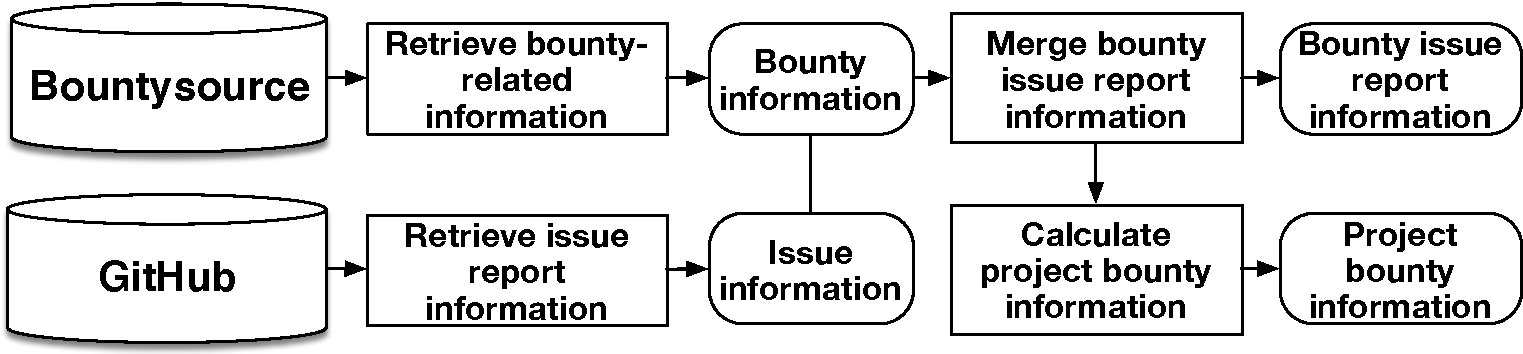
\includegraphics[width=9cm]{pics/datacollection/data_collection.pdf}
  \caption{An overview of our data collection process.}
  \label{overview}
  \vspace{-0.1in}

\end{figure}




All information about the bounties is stored on Bountysource and all details about issue reports and their corresponding projects are stored on GitHub. Hence, we collected data for our study along three dimensions: the bounty, the issue report, and the project.

\begin{figure}[t]
\centering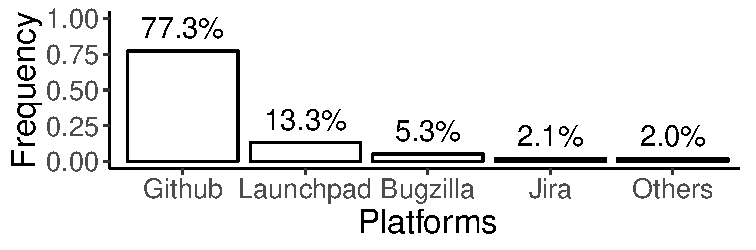
\includegraphics[width=0.8\columnwidth ]{pics/bg/RatioOfIssuesITS}
  \caption{The distribution of Bountysource bounties across the supported ITSs.}
  \label{RatioOfIssuesITS}
  \vspace{-0.1in}

\end{figure}

Figure~\ref{overview} presents an overview of our data collection process, which is broken down as follows:


\noindent\textbf{Step 1:} We retrieved the bounty and issue information from Bountysource using its official web API.\footnote{\url{https://bountysource.github.io/}} The bounty information includes the backers who proposed the bounty,  the proposed bounty value and the hunter who addressed the issue report. In addition, we collected basic information about the GitHub issue reports such as their id and URL.

\noindent\textbf{Step 2:} We retrieved the details of the issue reports, which are linked to Bountysource bounties by using the URL and id that we retrieved in step 1, from GitHub using its official web API.\footnote{\url{https://developer.github.com/v3/}} For example, we collected the description of the issue report, the creation date of the issue report, the comments that developers left under the issue, and the labels of the issue report.

\noindent\textbf{Step 3:} We calculated the corresponding project's bounty information for each collected bounty issue report, such as the number of total bounty issue reports of a project.



 \begin{table}[t]
   \centering
   \caption{Dataset description.}
     \begin{tabular}{p{24em}r}
    \hline
     Total number of bounties & 5,445 \bigstrut[t]\\
     Total number of claimed bounties & 2,402 \\
     Total bounty value & \$406,425 \\
     Total number of bounty hunters & 882 \\
     Total number of bounty backers & 2,534 \\
     Total number of issue reports & 3,509\\
     Total number of issue reports with multiple bounties & 795\\
     Total number of projects &  1,203 \bigstrut[b]\\
     \hline
     \end{tabular}%
   \label{tab:overviewOfGithub}%
   \vspace{-0.1in}

 \end{table}%


In total, we collected 5,445 bounties with a total value of \$406,425, together with their corresponding issue reports which were reported between Oct 19, 2012, and Oct 5, 2017. Table~\ref{tab:overviewOfGithub} gives a description of our dataset.


%We update the status of bounties for each issue at April 22, 2018 by Bountysource web-api\footnote{https://bountysource.github.io/}. \jy{Should introduce the distribution of issue-fixed day length to make the update reasonable?}

\begin{comment}
	
\begin{table}[ht]
  \centering
  \caption{Overview of the studied issues and their corresponding bounties. }
  \label{tab:overviewOfGithub}
  \begin{tabular}{|p{1cm}|p{1.6cm}|p{1.2cm}|p{1.2cm}|p{1.6cm}|p{1.3cm}|}
    \hline
    \textbf{\#Total Issue} & \textbf{\#Paid-out Issue} & \textbf{\#Total Bounty}& \textbf{\$Total Bounty}& \textbf{\$Paid-out Bounty}& \textbf{\#Bounty Hunter}\\
    \hline
   3,509&1,509  &5,445 &406,425 &218,824 &882  \\
    \hline
  \end{tabular}
\end{table}
\end{comment}






%=================== Preliminary study Here =================%
\section{Preliminary Study}
\label{prestudy}
\begin{figure}[t]
\centering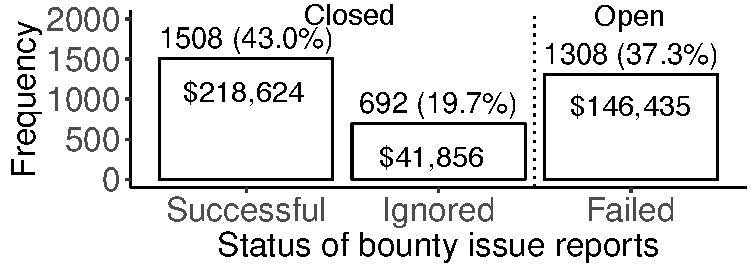
\includegraphics[width=0.8\columnwidth ]{pics/pre/pre_statusOfBounties.pdf}
\vspace{-0.1in}
\caption{The distribution of the possible statuses of bounty issue reports and their corresponding cumulative bounty value.}
\label{fig:pre_status_Bounties}
\vspace{-0.2in}

\end{figure}





In our preliminary study, we first present basic descriptive statistics
about the bounty: 1) the distribution of bounty issue reports across the possible statuses (i.e., successful, failed and ignored); 2) the distribution of the number of days between the reporting of the issue and its first bounty being proposed (i.e., \textit{days-before-bounty}); 3) the distribution of the frequency of bounties being used in projects (i.e., bounty-usage frequency).
From these statistics, we get a basic view of how bounties are used across projects. In addition, when a bounty issue report is closed and the bounty is paid out, we define this bounty issue report as addressed. We also calculate the issue-addressing likelihood against the bounty value and check the relationship between the issue-addressing likelihood and the bounty value.

%As we mentioned in Section~\ref{background}, in order to simplify our statement, we define three different bounties (i.e., the successful bounty, the failed bounty and the ignored bounty) according to three different status of the issue report.




\textbf{62.7\% of the bounty issue reports are closed, while the bounties in almost one-third of these closed issue reports remain unpaid with a value of \$41,856 in total.}
Figure~\ref{fig:pre_status_Bounties} shows the distribution of bounty issue reports across the three possible statuses. 37.3\% of the bounty issue reports are failed (i.e., open-unpaid). Although 62.7\% of the bounty issue reports were closed, almost one-third of their bounties were ignored (i.e., closed-unpaid). The total value of the ignored bounties (\$41,856) is ``frozen'' in the Bountysource platform unless someone claims the bounty.
In the rest of the paper, when we say the likelihood of an issue being addressed (i.e., issue-addressing likelihood), we only refer to the bounty issue reports that are successful (i.e., closed and paid out). We do not take the issue reports which were ignored into consideration because the hunters might not be driven by the bounty in such issue reports. We conducted a qualitative study of these closed-unpaid bounty issue reports to better understand them in Section \ref{rq4}.


\begin{figure}[t]
\centering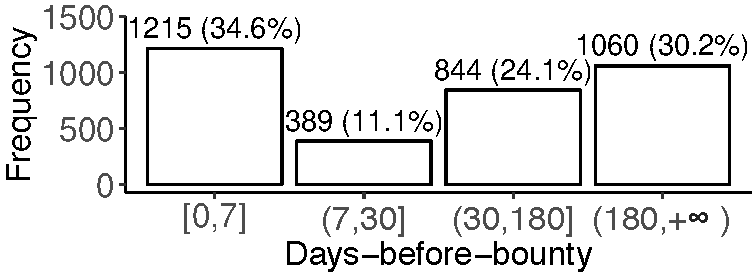
\includegraphics[width=0.8\columnwidth]{pics/pre/pre_delta_distribution_bounty}
\vspace{-0.1in}
\caption{The distribution of the number of days between the reporting of the issue and its first bounty being proposed (i.e., \textit{days-before-bounty}) in four different time ranges.}
\label{fig:pre_delta_distribution_bounty}
\vspace{-0.25in}

\end{figure}

\textbf{ 34.6\% of the bounties were proposed within 7 days from the creation of an issue report, while 30.2\% of bounties were proposed after more than 180 days.}
Figure~\ref{fig:pre_delta_distribution_bounty} shows the distribution of the \textit{days-before-bounty} metric in four continuous time ranges (i.e., 0 to 7 days, 8 days to 30 days, 31 days to 180 days, and more than 180 days). We observe that in 34.6\% of the issue reports their first bounty was proposed within 7 days after their creation, while in another 30.2\% of the issue reports their first bounty was proposed after more than 180 days since their creation.



 \begin{figure}[t]
   \centering
  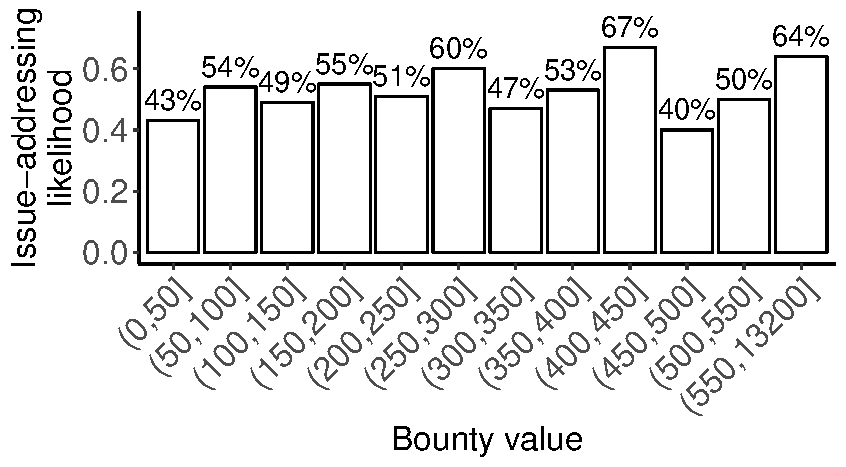
\includegraphics[width=0.8\columnwidth]{pics/pre/pre_i_value.pdf}
  \caption{The issue-addressing likelihood of the proposed bounty value ranges.}
  \label{fig:pre_v_value}
  \vspace{-0.1in}

\end{figure}

\textbf{More than half of the projects only used a bounty once, while two projects used bounties very frequently (more than 100 times)}. The distribution of the bounty-usage frequency of each project is skewed (with a variance of 57.02). 768 (65\%) projects used a bounty only once, 62 projects used a bounty at least 10 times and only 9 projects used a bounty more than 50 times.

%Because of the different bounty usage patterns in different projects, we investigate how the likelihood of an issue being addressed across projects with different bounty usage patterns in Section~\ref{rq1}.

%Figure~\ref{fig:preProjectEcdf} is the empirical cumulative distribution of the  bounty usage frequency for projects.



\textbf{The correlation between the bounty value and the issue-addressing likelihood is weak.} Figure~\ref{fig:pre_v_value} presents the issue-addressing likelihood of an issue report against the bounty value of an issue report. We do not observe patterns between them. The correlation between the bounty value and the issue-addressing likelihood is surprisingly weak~(0.14).

\rqbox{
Counter-intuitively, the correlation between the bounty value and the issue-addressing likelihood is weak. However, this low correlation may be due to the variation of the frequency of bounties that were used before in different projects and the timing of proposing the bounty.
}
Therefore, in Section~\ref{rq1} we investigate how the issue-addressing likelihood changes across projects with different bounty-usage frequencies. We study the relationship between the timing of proposing bounties and the issue-addressing likelihood in Section~\ref{rq2}.




%=================== RQ 1 Here =================%
\section{Studying how the issue-addressing likelihood changes across projects which have different bounty-usage frequencies}

\label{rq1}

Bounties are frequently used in some projects while rarely used in others (see Section~\ref{prestudy}). The frequency of using bounties in a project may reflect the degree of experience that the project has with bounties and may have an impact on the issue-addressing process.
Therefore, in this RQ, we investigate how the issue-addressing likelihood changes across different projects with different bounty-usage frequencies. Furthermore, we study the relationship of the issue-addressing likelihood with the bounty value and the project activities (e.g., creating pull requests).
With a better understanding of the bounty across different projects, we can provide insights on how to better use bounties.% for a wide range of projects.



\begin{figure}[t]
\centering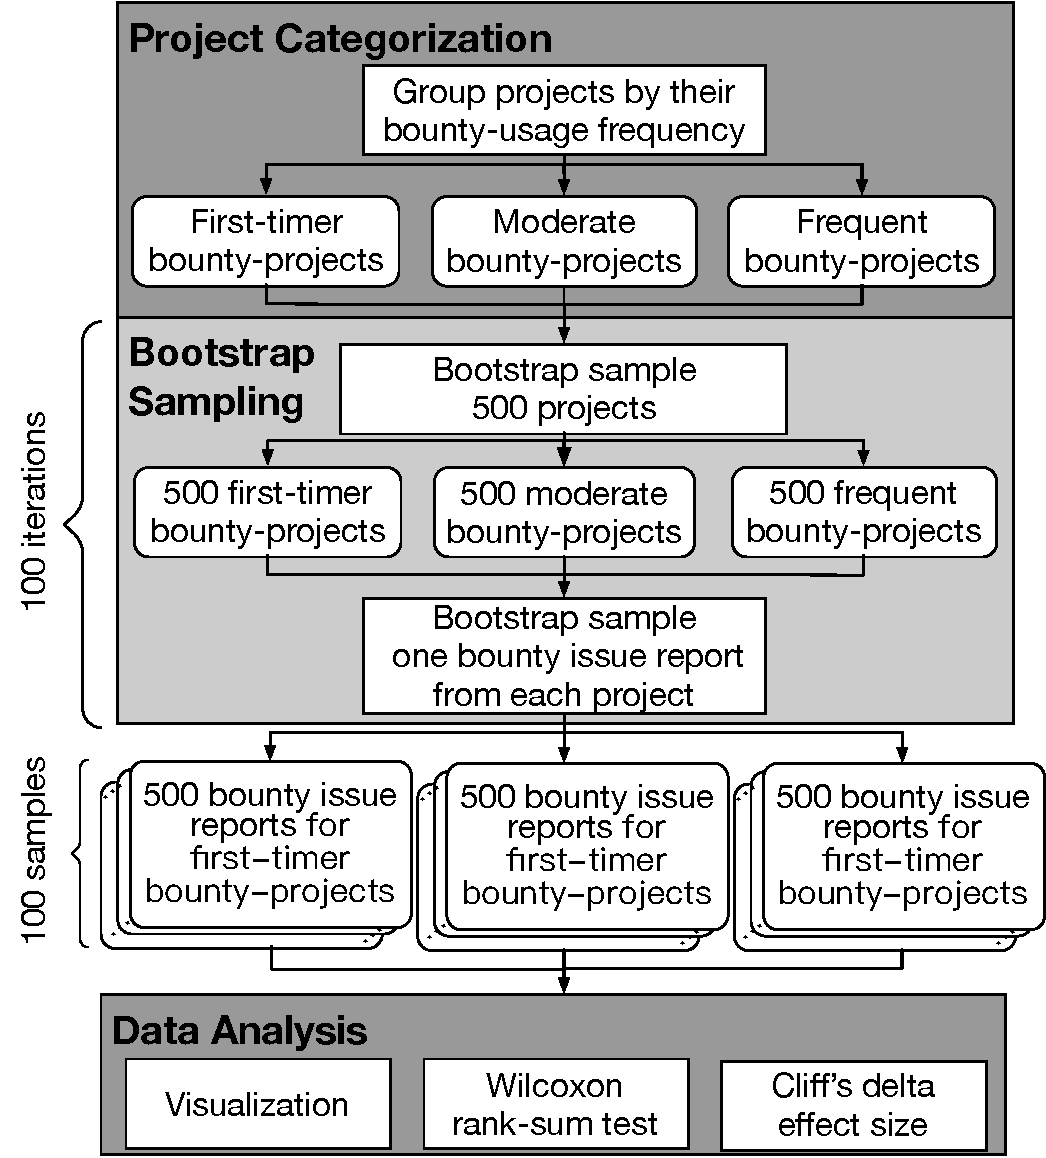
\includegraphics[width=\columnwidth ]{pics/rq1/new/approach}
\caption{An overview of our approach. }
\label{fig:rq1_approach}
\vspace{-0.2in}

\end{figure}

\noindent\textbf{Approach:} Figure~\ref{fig:rq1_approach} gives an overview of our approach. We elaborate on each step below.

\noindent\emph{\textbf{Project categorization:}} Given the variance (see Section~\ref{prestudy}) of the bounty-usage frequency for different projects, it is not advisable to study all the issue reports as one group when we study the bounties at the issue level. Therefore we categorize the projects into the following three groups:

\begin{enumerate}
    \item \textbf{First-timer bounty-projects:} Projects which have only one bounty issue report.
    \item \textbf{Moderate bounty-projects:} Projects which have 2 to 50 bounty issue reports.
    \item \textbf{Frequent bounty-projects:} Projects which have more than 50 bounty issue reports.
\vspace{-0.01in}
\end{enumerate}

It is important to study the bounties in the first-timer bounty-projects, since users of such projects may not have former bounty experience. Insights on the usage (e.g., how large of a bounty should be proposed?) and the impact (e.g., the issue-addressing likelihood) of bounties in these projects may benefit other projects which are new to using bounties. We grouped the projects that have more than 50 bounty issue reports as well since we assume that in such projects the community is more familiar with the use of bounties.
After grouping the projects into the above mentioned three groups we ended up with 768 (65\%) first-timer bounty-projects, 400 (34\%) moderate bounty-projects, and 9 (1\%) frequent bounty-projects. %Note that we study the impact of different thresholds for categorizing moderate bounty-projects and frequent bounty-projects in Section~\ref{sec:threats} and that find our observations still hold.


\noindent\emph{\textbf{Bootstrap sampling:}} After grouping the projects into the three groups, we used a bootstrap sampling approach to sample issue reports across projects. We used bootstrap sampling to reduce the bias that is caused by the unbalanced number of projects across the three groups. We first randomly sampled 500 projects from each group with replacement. Then we randomly sampled one bounty issue report from each sampled project, to avoid a bias towards projects with more issue reports than other projects in the same group. Hence, we sampled 500 bounty issue reports from each of the 3 project groups. To make our results more reliable, we repeated the sampling process 100 times with different random seeds. We ended up with 100 samples with 1,500 issue reports each (500 issue reports for each group).


\noindent\emph{\textbf{Data Analysis:}} For each sample, we calculated the issue-addressing likelihood across the three project groups and plotted the results. To compare the differences between two data distributions (e.g., the differences of the bounty values between successful and failed bounty issue reports), we used the Wilcoxon rank-sum test~\cite{bauer1972constructing}, which does not require the sample to be normally distributed. We consider the two distributions as significantly different when the p-value of the test is smaller than 0.05. Furthermore, we applied Cliff's delta $d$ \cite{long2003ordinal} effect size to quantify the magnitude of the difference. We use the following thresholds for $d$~\cite{romano2006appropriate}: $ \vert d \vert \leq$0.147 (negligible); 0.147 $ < \vert d \vert \leq $0.33 (small); 0.33 $ < \vert d \vert \leq $0.474 (medium); 0.474 $ < \vert d \vert  \leq $1 (large).


\begin{comment}
	
\begin{figure}[t]
\centering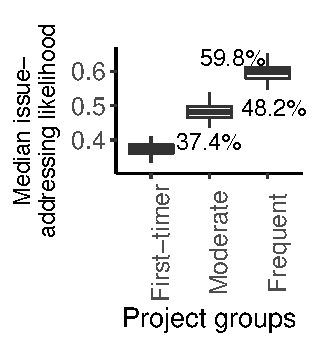
\includegraphics[width=\columnwidth]{pics/rq1/new/rq1_likelihood_ratio500}
\caption{The distribution of the median issue-addressing likelihood for each project group for 100 samples.}
\label{fig:rq1_likelihood_ratio500}
\vspace{-0.1in}
\end{figure}


\begin{figure}[t]
\centering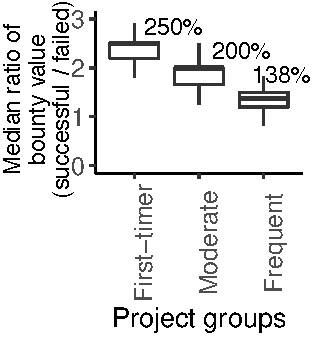
\includegraphics[width=\columnwidth]{pics/rq1/new/rq1_ratio_cp_ou500}
\caption{The distribution of the median ratio of the bounty value of successful bounty issue reports to the value of failed bounty issue reports against three project groups for 100 samples.}
\label{fig:rq1_ratio_cp_ou500}
\vspace{-0.1in}
\end{figure}

\end{comment}

\begin{figure}[t]
    \centering
    \begin{subfigure}[t]{0.45\columnwidth }
        \centering
        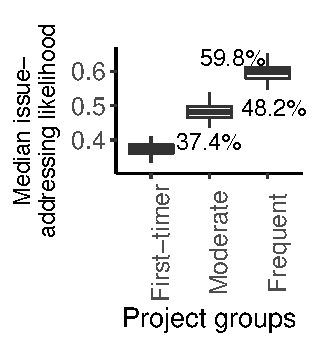
\includegraphics[width=\linewidth]{pics/rq1/new/rq1_likelihood_ratio500}
        \caption{}
		\label{fig:rq1_likelihood_ratio500}
    \end{subfigure}%
    ~
    \begin{subfigure}[t]{0.45\columnwidth}
        \centering
        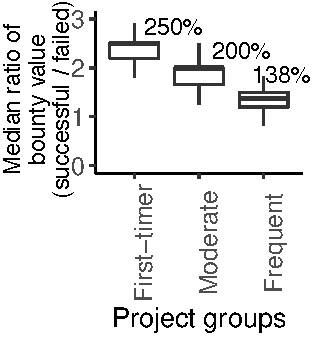
\includegraphics[width=\linewidth]{pics/rq1/new/rq1_ratio_cp_ou500}
        \caption{}
          \label{fig:rq1_ratio_cp_ou500}
    \end{subfigure}
    \vspace{-0.1in}
    \caption{The distribution of the median issue-addressing likelihood (a) and the distribution of the median ratio of the bounty value of successful bounty issue reports to the value of failed bounty issue reports (b) for each project group for 100 samples.
    }
    \vspace{-0.2in}
\end{figure}


\noindent\textbf{Results:}
\textbf{Bounty issue reports in projects which have a higher bounty-usage frequency are more likely to be addressed.} Figure~\ref{fig:rq1_likelihood_ratio500} shows the median issue-addressing likelihood for each project group. We observed a positive relationship between this likelihood and the bounty-usage frequency, which indicates that a bounty issue report is more likely to be addressed in a project with a higher bounty-usage frequency. Our statistical test shows that the issue-addressing likelihood is significantly different across these three groups of projects with a large effect size. One possible explanation is that the lower bounty-usage frequency of a project may indicate that the backers have less experience in proposing a bounty (e.g., at the proper time with a proper value) and the hunters react to bounties less actively than in projects with a higher bounty-usage frequency.



\textbf{The successful bounty issue reports have a relatively higher bounty value than failed bounty issue reports, particularly in the first-timer bounty-projects.}
Figure~\ref{fig:rq1_ratio_cp_ou500} shows that the median ratio (the bounty values of successful reports compared to those of failed reports) is larger than 1 in all 3 project groups. In other words, the successful bounty issue reports have higher bounty values than the failed bounty issue reports. In addition, comparing the ratio across project groups, the first-timer bounty-projects have the largest ratio (2.5) among the three groups, indicating that developers may want more money to address an issue in first-timer bounty-projects than in other projects. Our statistical test results shows that the differences in bounty value between successful and failed bounty issue reports are significant (p-value $<$ 0.05) in the first-timer bounty-projects for all samples with a non-negligible Cliff's delta effect size (72\% samples have a small effect size and 28\% samples have a medium effect size).
In 97\% of the samples of the moderate bounty-projects, the bounty value of successful issue reports is significantly higher than that of failed issues (with a non-negligible effect size in 77\% of the cases).
For the frequent bounty-projects, in 92\% of the samples, the differences were not statistically significant.


\begin{comment}
 \begin{table}[t]
   \centering
   \caption{The comparison of the bounty values between successful bounty issue reports and failed bounty issue reports across three project groups over 100 samples. For example, the differences in bounty value between successful bounty issue reports and failed bounty issue reports in first-timer projects are statistically significant across all the samples (i.e., 100\%). }
     \begin{tabular}{ccccc}
     \toprule
     \multicolumn{1}{c}{} \makecell{\textbf{Bounty-project}\\\textbf{group}}&  \multicolumn{1}{c}{\makecell{\textbf{Wilcoxon}\\\textbf{rank-sum test}}} & \multicolumn{3}{p{3.5cm}}{\textbf{\rule{10pt}{0pt}Cliff's Delta effect size}} \bigstrut\\
    \hline
      & Significant & \multicolumn{1}{p{1.1cm}}{Negligible} & \multicolumn{1}{p{0.1cm}}{Small} & \multicolumn{1}{p{1cm}}{Medium} \bigstrut\\
     \hline
     \textbf{First-timer} &  100\%      & \rule{9pt}{0pt} 0\%     & \rule{3pt}{0pt} 72\%    &\rule{3pt}{0pt}  28\% \\
     \hline
     \textbf{Moderate}&  \rule{4pt}{0pt}97\%        & \rule{9pt}{0pt}23\%    & \rule{5pt}{0pt}76\%    & \rule{9pt}{0pt}1\% \\
     \hline
     \textbf{Frequent} &  \rule{4pt}{0pt}24\%      & \rule{9pt}{0pt}92\%    & \rule{9pt}{0pt}8\%     & \rule{9pt}{0pt}0\% \\
     \hline

     \end{tabular}%
   \label{tab:rq2_value_comparison}%
   \vspace{-0.1in}

 \end{table}%
\end{comment}

One possible explanation is that first-timer bounty-projects may not be as active as moderate and frequent projects. Therefore, backers would be required to propose bounties with higher values to attract enough attention from the community for addressing issues. To investigate this explanation, we examined the activity of the projects in terms of the number of pull requests, issue reports, and commits. Figure~\ref{fig:rq1_activity} shows the distributions of the occurrences of these three activities in each project group.
%The projects in the category with more bounty-usage frequency have more activities.
\textbf{Projects with fewer bounty issue reports are usually less active (in terms of the number of pull requests, issue reports, and commits) than projects with more bounty issue reports.} Another possible explanation is that the backers in the first-timer bounty-projects have no experience in proposing bounties and sometimes overestimate the value of addressing an issue report. In this situation, the overestimated bounty issue reports may attract more attention from the community due to their ``easy money'' and get addressed easier.



\begin{figure}[t]
\centering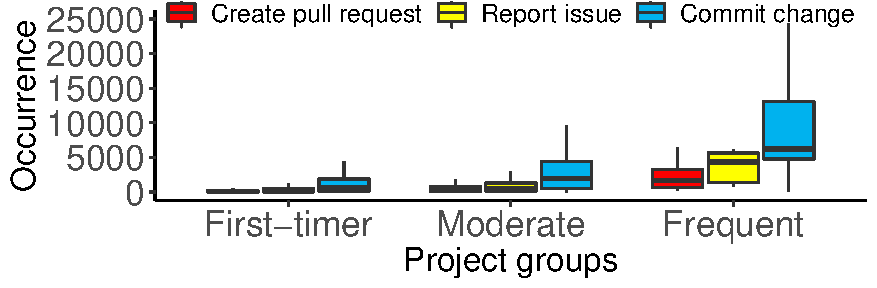
\includegraphics[width=\columnwidth]{pics/rq1/new/rq1_activity}
\caption{The distributions of the occurrences of three activities (i.e., the create pull request, the report issue and the commit change) in each project group.}
\label{fig:rq1_activity}
\vspace{-0.2in}

\end{figure}


\rqbox{The issue-addressing likelihood is higher in projects which used bounties more frequently. Successful bounty issue reports have higher bounty values than failed bounty issue reports in the projects which used bounties less frequently.}



%=================== RQ 2 Here =================%
\section{Studying the relationship between the timing of proposing a bounty and the issue-addressing likelihood}
\label{rq2}

In Section~\ref{prestudy}, we observe different patterns for the timing of proposing bounties, which may have different relationships with the issue-addressing likelihood. In this section, we investigate the relationship between the timing of proposing bounties and the issue-addressing likelihood. With a better understanding of the relationship, we can provide insights into how to improve the timing of proposing a bounty.

\textbf{Approach:}
We use the same data (100 samples of 1,500 issue reports for each sample) as RQ1. For each sample, we grouped data into four timing ranges based on the number of elapsed days between the creation of an issue report and the proposal of its first bounty(i.e., \textit{days-before-bounty}). We defined the four timing ranges as follows:
\begin{enumerate}
    \item \textbf{[0,7]:} the first bounty was proposed within seven days after the issue was reported.
    \item \textbf{(7,30]:} the first bounty was proposed between 7 and 30 days after the issue was reported.
    \item \textbf{(30,180]:} the first bounty was proposed between 30 and 180 days after the issue was reported.
    \item \textbf{(180,$\infty$):} the first bounty was proposed after 180 days after the issue was reported.
\end{enumerate}

Then we calculate the issue-addressing likelihood across the timing ranges for each sample to study the relationship between the timing and issue-addressing likelihood.
To further study the relationship between the issue-addressing speed and the timing, we also calculate the time it takes to close the issue report after the first bounty is proposed (i.e., \textit{time-to-close}) in each timing range for each sample.
Furthermore, we also study the timing in terms of different project groups for each sample.
\begin{comment}
	
\begin{figure}[t]
\centering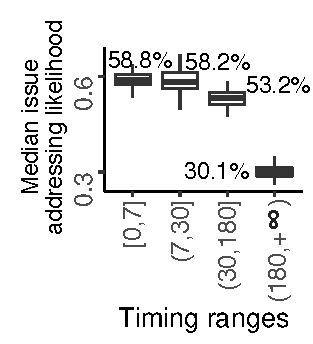
\includegraphics[width=\columnwidth]{pics/rq2/new/rq2_delta_ratio}
  \caption{The distribution of the median issue-addressing likelihood across the  timing ranges for the 100 studied samples.}
  \label{fig:rq2_delta_ratio}
  \vspace{-0.1in}

\end{figure}
\begin{figure}[t]
\centering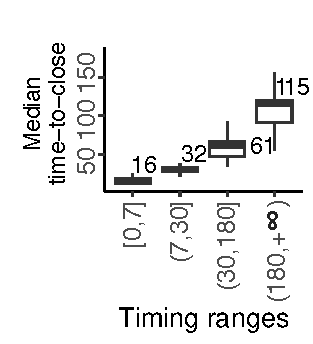
\includegraphics[width=\columnwidth]{pics/rq2/new/rq2_closeday_deltaday}
  \caption{The distribution of the median time to close an issue report (i.e., \textit{time-to-close}) for each timing range for 100 samples.}
  \label{fig:rq2_closeday_deltaday}
  \vspace{-0.1in}
\end{figure}
\end{comment}

\begin{figure}[t]
    \centering
    \begin{subfigure}[t]{0.5\columnwidth }
        \centering
        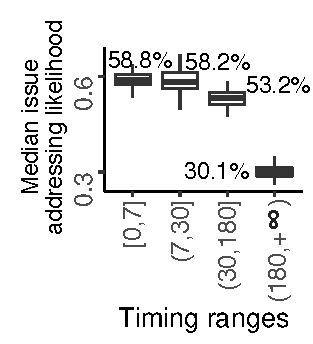
\includegraphics[width=\linewidth]{pics/rq2/new/rq2_delta_ratio}
        \caption{}
		\label{fig:rq2_delta_ratio}
    \end{subfigure}%
    ~
    \begin{subfigure}[t]{0.5\columnwidth}
        \centering
        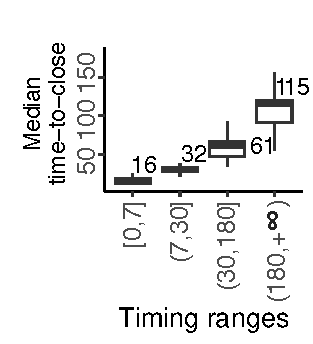
\includegraphics[width=\linewidth]{pics/rq2/new/rq2_closeday_deltaday}
        \caption{}
          \label{fig:rq2_closeday_deltaday}
    \end{subfigure}
    \vspace{-0.1in}
    \caption{The distribution of the median issue-addressing likelihood (a) and the  distribution of the median time to close an issue report (i.e., \textit{time-to-close}) (b) across the  timing ranges for the 100 studied samples.
    }
\end{figure}
\begin{figure}[t]
\centering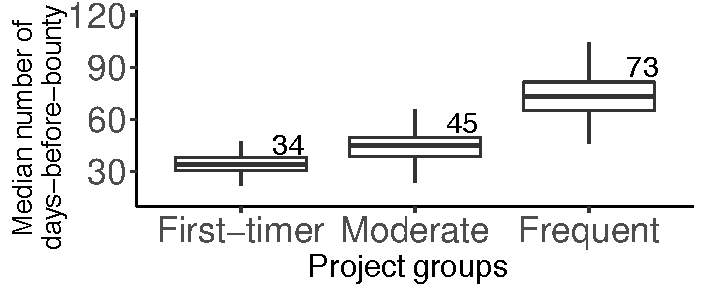
\includegraphics[width=0.8\columnwidth]{pics/rq2/new/rq2_medianDeltaTime.pdf}
  \caption{The distribution of the median number of days between the creation of the issue report and the proposed of the first bounty to the bounty is proposed (i.e., \textit{days-before-bounty}) across different project groups for 100 samples.}
  \label{fig:rq2_medianDeltaTime}
  \vspace{-0.15in}

\end{figure}




\noindent\textbf{Results:}\textbf{ In general, issue reports for which bounties were proposed earlier have a higher likelihood of being addressed.} Figure~\ref{fig:rq2_delta_ratio} shows the distribution of the median issue-addressing likelihood across the timing ranges over 100 samples. We calculated the Wilcoxon rank-sum test and Cliff's delta test to measure the differences between two distributions. The results show that there is no significant difference between the distributions of ``[0,7]'' and ``(7,30]'' while there exist significant differences with large effect sizes for the other two distributions.
The likelihood is getting smaller as the \textit{days-before-bounty} gets larger, especially for the issue reports in which bounties are proposed after 180 days where the likelihood drops to 30\%.

One possible explanation is that as time progresses, the risk of a report becoming obsolete exists, leaving the issue report unaddressed even after a bounty is proposed.
For example, an issue report\footnote{\url{https://github.com/bhdouglass/uappexplorer/issues/69}} that was created on Feb 4, 2016 in the \code{uappexplorer} project requested a new feature for an Ubuntu Phone Application.
The owner of the application and another developer both showed great interest in this issue. Because of the lack of time, the feature was never added. A bounty of \$5 was proposed\footnote{\url{%https://www.bountysource.com/issues/30521886-allow-comments-on-wishlist-items/backers
http://bit.ly/2Q3BIns}} after almost one year (i.e., on Jan 12, 2017).
However, the issue report was closed because Ubuntu Phone was no longer used making the issue report obsolete. Because of the low value, the bounty was not refundable. In other words,\textbf{ backers carry the risk of wasting their money by proposing small bounties on such long-standing issue reports.}

Another possible reason for the lower issue-addressing likelihood of the issue reports for which bounties were proposed later is the potential difficulty of such issue reports.
Figure~\ref{fig:rq2_closeday_deltaday} shows the median time that was taken to close issues (i.e., \textit{time-to-close}) across each timing range. We observe that the issue reports in which bounties were proposed later took more time to be addressed.




\textbf{Backers proposed bounties earlier in the first-timer bounty-projects.}
Figure~\ref{fig:rq2_medianDeltaTime} presents the distribution of the median value of the \textit{days-before-bounty} metric across the project groups for each sample. The median \textit{days-before-bounty} is 34, 45 and 73 for each project group, respectively.
We calculated the Wilcoxon rank-sum test and Cliff's delta $d$ effect size to measure the differences of distributions between the first-timer bounty-projects and the moderate bounty-projects, the moderate bounty-projects and the frequent bounty-projects, respectively. The result shows that any two pairs of distributions are significantly different with large Cliff's delta effect sizes, indicating that the \textit{days-before-bounty} is higher in projects with a higher bounty-usage frequency.
One explanation is that the activity of first-timer bounty-project is lower (see Figure~\ref{fig:rq1_activity}), which may encourage backers to propose a bounty earlier to attract developers to get an issue addressed.

%For example, Figure~\ref{fig:rq1_activity} shows that the first-timer projects have the smallest number of forks among all three project groups.



\rqbox{In general, issue reports for which bounties were proposed earlier have a higher likelihood of being addressed. In addition, the risk of losing money exists for backers who propose small bounties for long-standing issue reports.
}



%=================== RQ 3 Here =================%

\section{Using a logistic regression model to study the relationship between the studied factors and the issue-addressing likelihood}

\label{rq3}

%Developers and users can use a bounty to motivate developers to address an issue report. However, it still remains unclear how bounties affect the issue-addressing process.



In the previous sections, we studied the relationship between the issue-addressing likelihood, the bounty-usage frequency and the timing of proposing a bounty. However, there may exist more factors that potentially affect the issue-addressing likelihood. In this section, we conduct a deeper study on the relationship between other factors and the issue-addressing likelihood.
With a better understanding of this relationship, we can provide insights into how to use a bounty to improve the issue-addressing process.

\begin{figure*}[t]
\centering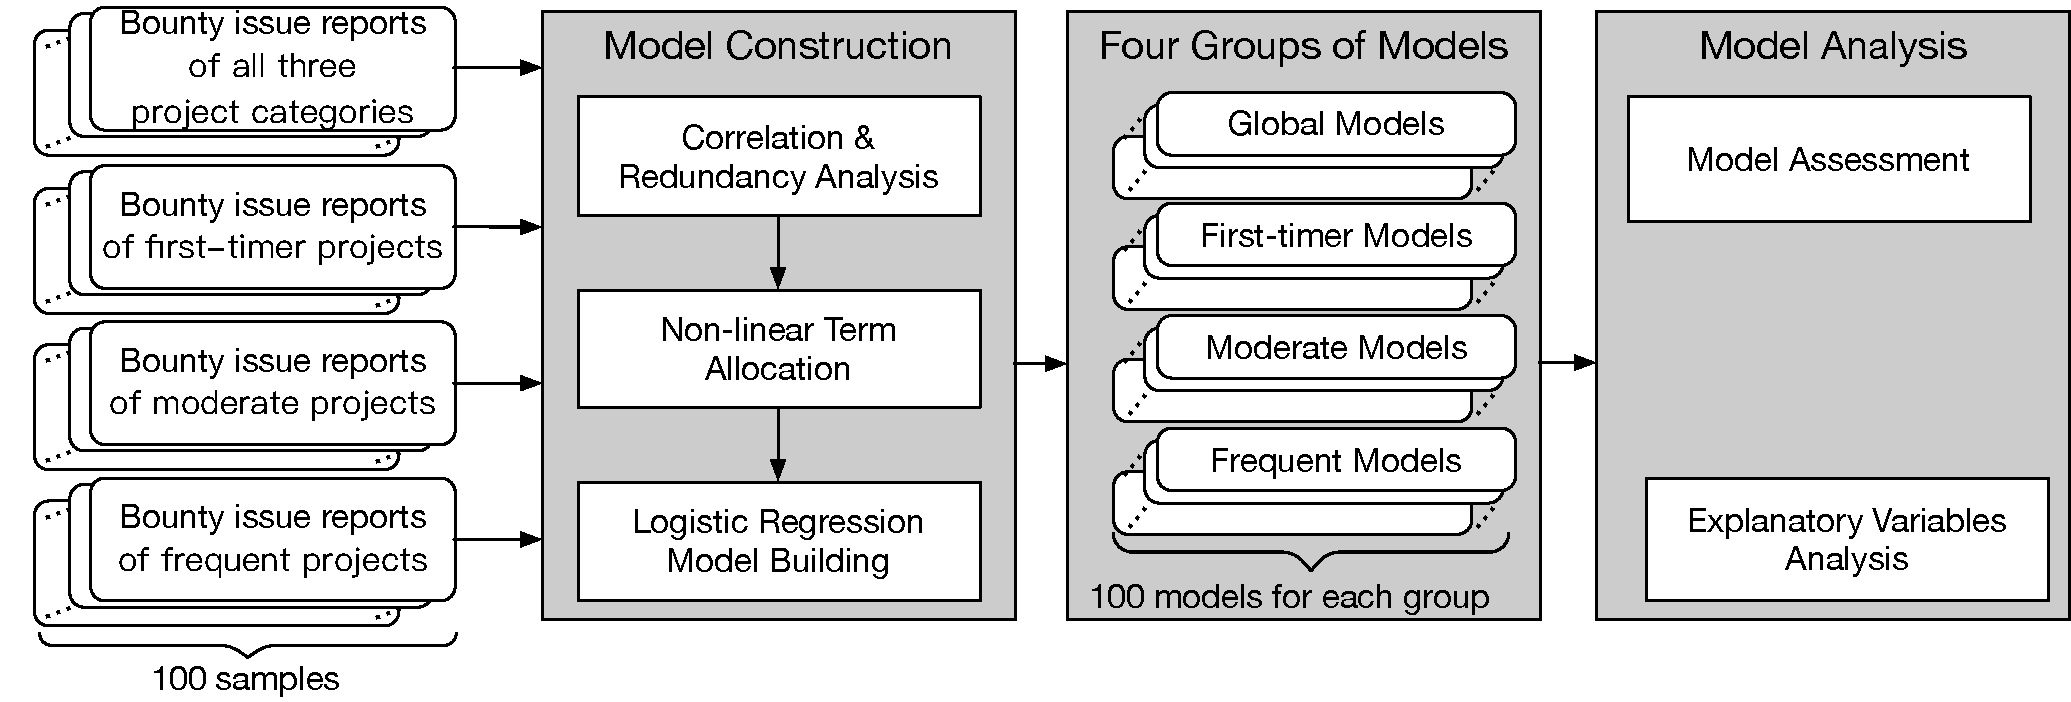
\includegraphics[width=17cm]{pics/rq3/rq3flow}
\vspace{-0.2in}
\caption{An overview of the model construction and analysis.}
\label{fig:rq3_flow}
\vspace{-0.1in}
\end{figure*}

\subsection{Approach}
In this section, we use the same data as in Section~\ref{rq1} to build logistic regression models to investigate the relationship between the studied factors and the issue-addressing likelihood.
Firstly, we build models on the entire set of bounty issue reports to understand the global relationship (referred to as the \textbf{global model}). Secondly, as we can see in Section~\ref{rq1}, the issue-addressing likelihood changes across project groups (i.e., the first-timer bounty-projects, the moderate bounty-projects, and the frequent bounty-projects). To understand the relationship within each project group, we build logistic regression models on the bounty issue reports of each group separately. To condense our writing, we refer to the model for the first-timer, moderate, and frequent bounty-projects as the \textbf{first-timer model}, \textbf{moderate model}, and \textbf{frequent model}, respectively.
We use the logistic regression modeling technique since it is a robust and highly interpretable technique, which has been applied successfully in software engineering before~\cite{wang2017understanding,mcintosh2016empirical}.
Figure~\ref{fig:rq3_flow} gives an overview of our approach.
Below, we elaborate on the studied factors, the processes of the model constructions, and the analysis of our models.

\subsubsection{Studied factors}
\begin{table*}[]
\centering
\footnotesize
\caption{The description of and rationale for the factors in the \emph{Issue report basic} and the \emph{Issue report bounty} dimensions. The factors which are marked with `*' are  time-dependent factors which are calculated at the time when the bounty is proposed}
\label{tab:factors1}

     \begin{tabular}{p{12em}p{29em}p{19em}}
     %\toprule
     \toprule
     \multicolumn{1}{l}{\textbf{Factor name}}  & \textbf{Description} & \multicolumn{1}{p{19em}}{\textbf{Rationale}} \\

     \midrule
     \multicolumn{3}{p{30em}}{\textbf{Issue report basic}}\\
     \midrule
      I\_content\_len*                  & The length of an issue report and its comments (in characters).  &\multirow{5}[-3]{19em}{\parbox{19em}{These factors reflect the amount of supportive information that an issue report has. Issue reports with more supportive information may help developers to address them.}} \\
%\cline{1-2}
     I\_code\_len* & The total length of the code snippets in an issue report and its comments (in characters). &  \\
%\cline{1-2}
      I\_code\_proportion*              & The proportion of code in an issue report and comments (i.e., $\frac{I\_code\_len}{I\_content\_len}$).\makecell{ \rule{0pt}{12pt} } &  \\
      \midrule
    I\_link\_cnt*                     & The number of links in an issue report and its comments. & \multirow{5}[-4]{19em}{\parbox{19em}{The discussion activities reflect the popularity of an issue report, which may have a relationship with the issue-addressing likelihood.}} \\
%\cline{1-2}
     I\_img\_cnt*                      & The number of images in an issue report and its comments. &  \\

%\cline{1-2}
     I\_cmnt\_cnt                     & The number of comments that an issue report received. & \\
%\cline{1-2}
	I\_participant\_cnt* & The number of participants in the discussion of an issue. & \\
%\cline{1-2}
     I\_cmnt\_per\_day\_mean* & The mean number of comments per day for an issue report. &  \\
 \midrule
     \textbf{Issue report bounty} & \multicolumn{2}{l}{\textbf{Description (d) - Rationale (r)}} \\
     \midrule
     I\_B\_days\_before\_bounty*  & \multicolumn{2}{p{48em}}{d: The number of days between the creation of an issue report and its first bounty.\newline r: Different timing of proposing bounties have relationship with the issue-addressing likelihood.} %\bigstrut
     \\
     %\hline
     %\midrule
      I\_B\_total\_value & \multicolumn{2}{p{48em}}{d: The total bounty value of the issue report. \newline r: A higher bounty may attract more developers.} \\
     %\midrule
     %\hline
      I\_B\_cnt    &  \multicolumn{2}{p{48em}}{d: The number of bounties that a bounty issue report has. \newline r: A higher number indicates that more backers are interested in getting this issue  addressed.} \\
      %\hline
     %\midrule
     I\_B\_has\_label  &  \multicolumn{2}{p{48em}}{d: Whether a bounty issue report is tagged with a bounty label. \newline r: A bounty label could help draw attention from the community, which may impact the issue-addressing likelihood. } \\
     %\hline
     %\midrule
      I\_B\_timing\_range*   & \multicolumn{2}{p{48em}}{d: The range of the timing of proposing the first bounty.                                                                                 \newline r: The timing of proposing a bounty has a relationship with the issue-addressing likelihood (see Section~\ref{rq2}).} \\
     \bottomrule
     %\hline
%\multicolumn{3}{l}{\textbf{Note:} The factors with `*' are collected at the time of proposing the first bounty for the issue report.}\bigstrut\\
     \end{tabular}%
     \vspace{-0.1in}
 \end{table*}%

\begin{table*}[ ]
\centering
%\tiny
\caption{The description of and rationale for the factors in the \emph{Project bounty} and the \emph{Backer experience} dimensions. The factors which are marked with `*' are  time-dependent factors which are calculated at the time when the bounty is proposed}
\label{tab:factors2}

     \begin{tabular}{p{10em}p{29em}p{21em}}
     \toprule
     \multicolumn{1}{l}{\textbf{Factor name}}  & \textbf{Description} & \multicolumn{1}{p{21em}}{\textbf{Rationale}} \\
     \midrule
     \multicolumn{3}{p{30em}}{\textbf{Project bounty}}\\
     \midrule
     P\_B\_I\_cnt*                     &  The total number of issue reports with at least one bounty of a project.  & \multicolumn{1}{r}{\multirow{5}[-5]{21em}{\parbox{21em}{These five factors reflect the bounty activity of the project. A different level of activity may have a different impact on the issue-addressing likelihood in the project.}}} \\
%\cline{1-2}
     P\_B\_paid\_cnt* & The total number of paid bounty issue reports of a project. &  \\
%\cline{1-2}
     P\_B\_open\_cnt*     &  The number of open bounty issue reports of a project.  &\\
%\cline{1-2}
     P\_B\_paid\_proportion* & The proportion of paid bounty issue reports of a project. &  \\
%\cline{1-2}
     P\_B\_total\_value* & The total value of the bounties of a project. &  \\
\midrule
      P\_B\_usage\_group                    &   The group of projects.                                                                                  & \multicolumn{1}{p{21em}}{Different groups of projects have different issue-addressing likelihoods (see Section~\ref{rq1}).} \\
     \midrule
     \multicolumn{3}{p{30em}}{\textbf{Backer experience}}\\
     \midrule
     Backer\_exp\_B\_median/sum/max\_value* & The median/sum/max value of bounties which the backers of this bounty have ever proposed in the past. & \multicolumn{1}{r}{\multirow{2}[1]{21em}{\parbox{21em}{Bounties from a backer who has proposed bounties often, or proposed high-value bounties in the past may attract more attention from developers.}}} t\\
%\cline{1-2}
     Backer\_exp\_B\_median/sum/max\_cnt* & The median/sum/max number of bounties which the backers of this bounty have ever proposed in the past. &  \\
     \midrule
     Backer\_role\_any\_insider* & Whether any of the backers who has ever contributed to the project.  & \multicolumn{1}{r}{\multirow{2}[1]{21em}{\parbox{21em}{A backer who has ever interacted with the project before may help the bounty attract more attention from the community.}}} \bigstrut\\
%\cline{1-2}
Backer\_role\_have\_reporter* & Whether the issue reporter is one of the backers for that issue report.\\
     \midrule

%\multicolumn{3}{l}{\textbf{Note:} The factors with `*' are collected at the time of proposing the first bounty for the issue report.}\\
     \end{tabular}%
\vspace{-0.2in}
 \end{table*}%

We consider 27 factors along 4 dimensions:
\begin{enumerate}
    \item \textbf{Issue report basic:} Eight factors which can estimate the length and the popularity of an issue report.
    \item \textbf{Issue report bounty:} Five factors which describe the bounty usage within a bounty issue report.
    \item \textbf{Project bounty:} Six factors which reflect the bounty usage within a project.
    \item  \textbf{Backer experience:}  Eight factors which capture the bounty experience of the backers of a bounty issue report.
\vspace{-0.01in}
\end{enumerate}

Table~\ref{tab:factors1} and Table~\ref{tab:factors2} summarize the description of and rationale behind the studied factors. The factors which are marked with `*' are time-dependent factors which are calculated at the time when the bounty is proposed.
Note that the factors in the project bounty, issue report basic, and backer experience dimensions cannot be changed by a backer who wants to propose a bounty. Hence we include these factors as control factors in our models.



\subsubsection{Model construction}
Similar to prior studies~\cite{gopi:2017,wang2017understanding,mcintosh2016empirical,kabinna2018examining}, we first removed correlated and redundant factors by using the Spearman rank correlation test and the redundancy analysis to avoid multicollinearity. We ended up with three factors in the project bounty dimension, six factors in the issue report basic dimension, four factors in the issue report bounty dimension, and three factors in the backer experience dimension.
Then we added non-linear terms in the model to capture the more complex relationship in the data by employing restricted cubic splines~\cite{Harrell:2006}.
Finally, we used the \code{rms} \code{R} package\footnote{\url{https://cran.r-project.org/web/packages/rms/index.html}} to implement our logistic regression models (i.e., the first-timer, moderate, frequent, and global models) based on 100 samples and ended up with 400 models. See our appendix~\cite{appendix} for more details about our model construction.

\subsubsection{Model analysis}
For each logistic regression model, we used the Area Under the Receiver Operating Characteristic Curve (i.e., \textit{AUC}) and a bootstrap-derived approach \cite{efron1986biased} to assess the explanatory power of the models following prior studies~\cite{mcintosh2016empirical,wang2017understanding,kabinna2018examining}. The AUC ranges from 0 to 1, with 0.5 being the performance of a random guessing model and a higher AUC meaning that the model has a higher ability to capture the relationships between the  explanatory factors and the response factor. To check whether the models are not overfitted, we calculate their \textit{optimism} values using a bootstrap-derived approach (with a small optimism value indicating that the model is not overfitted). 

To study the impact of each factor on the issue-addressing likelihood, we used the \textbf{anova} function in the R \textbf{rms} package to compute the Wald $\chi^2$ value.
The larger the Wald $\chi^2$ value of a factor is, the larger the impact of the factor on the issue-addressing likelihood.
We computed the Wald $\chi^2$ value for each factor for each model and used the median Wald $\chi^2$ value of each factor within a group to represent the impact of that factor in that group. %For the Wald $\chi^2$ value of factors in each group of models, please see the in Appendix\jy{ will add the specific section of appendix later}.

In addition, to further understand how a factor influences the value of the response variables, we used the \textbf{Predict} function in the \textbf{rms} R package to plot the estimated issue-addressing likelihood against a factor. Since all models across 100 samples showed similar patterns of influence for the factors, we randomly selected a sample as an example to build models and visualize the results (see Figure~\ref{fig:rq3_trend_global} and Figure~\ref{fig:rq3_trend_two}).
The analysis allows us to further understand how a factor affects the issue-addressing likelihood. %We hold the other factors at their median values when exploring a specific factor.
For the detailed results of our model analysis, such as the $\chi^2$ values, we refer the reader to our online appendix~\cite{appendix}.

%\begin{figure}[t]
%\centering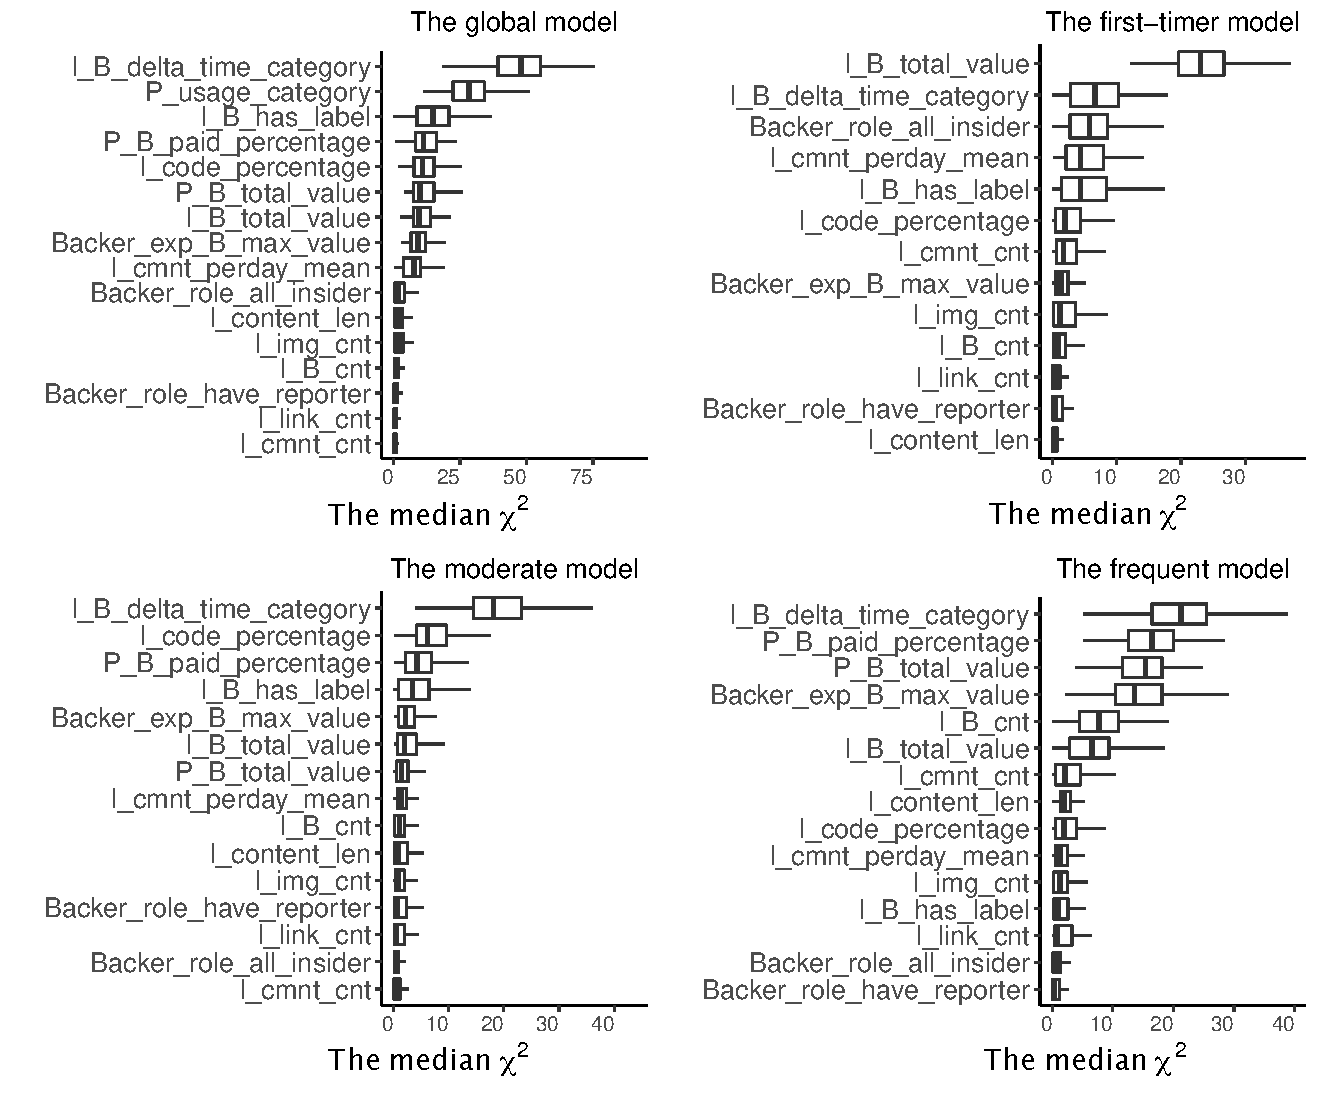
\includegraphics[width=\columnwidth]{pics/rq3/rq3_altogether}
%\caption{The distribution of the median Wald $\chi^2$ value of each factor in 100 samples for each group of models.}
%\label{fig:rq3_altogether}
%\end{figure}


\begin{figure}[t]
\centering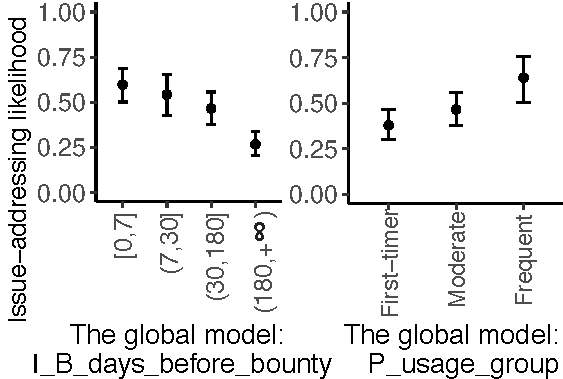
\includegraphics[width=0.7\columnwidth ]{pics/rq3/rq3_trend_global}
\caption{The plots show the relationship between the studied factors and the issue-addressing likelihood in the global models in the selected sample. For each plot, we adjusted all factors except the studied factor to their median value in the model and recomputed the issue-addressing likelihood. The grey area represents the 95\% confidence interval.}
\vspace{-0.1in}
\label{fig:rq3_trend_global}
\end{figure}

\begin{comment}
	
\begin{figure}[t]
\captionsetup[subfigure]{labelformat=empty}
    \centering
    \begin{subfigure}[t]{\columnwidth }
        \centering
        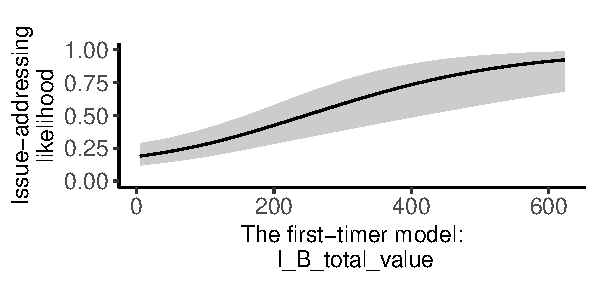
\includegraphics[width=\linewidth]{pics/rq3/split/rq3_trendCat1}
        \caption{}
		\label{fig:rq3_trendCat1}
    \end{subfigure}%

  \vspace{-0.2in}
    \begin{subfigure}[t]{\columnwidth}
        \centering
        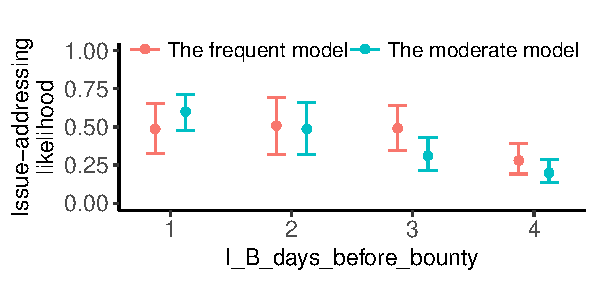
\includegraphics[width=\linewidth]{pics/rq3/split/rq3_trendMerge}
        \caption{}
          \label{fig:rq3_trendMerge}
    \end{subfigure}
  \vspace{-0.3in}
    \caption{The plots show the relationship between the studied factors and the issue-addressing likelihood in the first-timer, moderate and frequent models in the selected sample. For each plot, we adjusted all factors except the studied factor to their median value in the model and recomputed the issue-addressing likelihood. The grey area represents the 95\% confidence interval.
    }
    \label{fig:rq3_trend_two}
  \vspace{-0.1in}
\end{figure}

\end{comment}
\begin{figure}[t]
\centering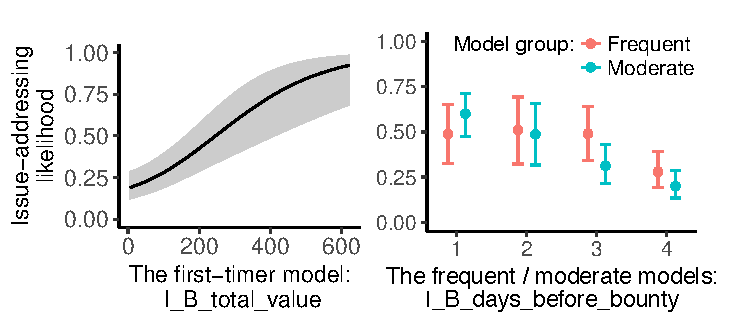
\includegraphics[width=1.03\columnwidth ]{pics/rq3/split/rq3_trendMergeMerge}
\caption{The plots show the relationship between the studied factors and the issue-addressing likelihood in the first-timer, moderate and frequent models in the selected sample. For each plot, we adjusted all factors except the studied factor to their median value in the model and recomputed the issue-addressing likelihood. The grey area represents the 95\% confidence interval.}
\vspace{-0.1in}
\label{fig:rq3_trend_two}
\end{figure}

 % Table generated by Excel2LaTeX from sheet 'Sheet1'
 \begin{table}[t]
   \centering
   \caption{The two most important factors, the median AUC and the median optimism (Opt.) values for our models.}
     \begin{tabular}{lp{8em}lcc}
     \toprule
     \textbf{Group} & \multicolumn{2}{c}{\rule{-14pt}{0pt} \textbf{Factor importance}} & \multicolumn{2}{c}{\rule{-11pt}{0pt}\textbf{Median}}\\
     \midrule
           & \multicolumn{1}{c}{\rule{-13pt}{0pt}$1^{st}$} & \multicolumn{1}{c}{\rule{-14pt}{0pt} $2^{nd}$} &  AUC & Opt.\\
     \midrule
     Global  &\rule{-13pt}{0pt} \textit{I\_B\_timing\_range} &\rule{-14pt}{0pt} \textit{P\_B\_usage\_group} &\rule{-11pt}{0pt} 0.72 & 0.02 \\
     
First-timer &\rule{-13pt}{0pt} \textit{I\_B\_total\_value} &\rule{-14pt}{0pt} \textit{I\_B\_timing\_range} &\rule{-11pt}{0pt} 0.74 & 0.03 \\

  Moderate &\rule{-13pt}{0pt} \textit{I\_B\_timing\_range} &\rule{-14pt}{0pt} \textit{I\_code\_proportion} &\rule{-11pt}{0pt} 0.71& 0.04 \\

   Frequent &\rule{-13pt}{0pt} \textit{I\_B\_timing\_range} &\rule{-14pt}{0pt} \textit{P\_B\_paid\_proportion} &\rule{-11pt}{0pt} 0.81 & 0.03 \\
     \bottomrule
     \end{tabular}%
   \label{tab:top3impFactors}%
   \vspace{-0.2in}
 \end{table}%


\subsection{Results}
\textbf{Our models explain our dataset well and have a reliable performance.} The median AUCs for each group of models are all at least 0.71 (see Table~\ref{tab:top3impFactors}), which indicates that our models explain the dataset well and the low median optimism values (between 0.02 and 0.04) indicate that our models do not overfit the dataset.

\textbf{In the global view, the timing of proposing the bounties and the bounty-usage frequency are the top two most important factors that impact the issue-addressing likelihood.} Table~\ref{tab:top3impFactors} shows the top two important factors (ranked by median Wald's $\chi^2$ value) in the global models across 100 samples.
\textit{I\_B\_timing\_range} (i.e., the range of the timing of proposing bounties) and \textit{P\_B\_usage\_group} (i.e., the group of projects' bounty-usage frequency) are the most important factors which contribute the most explanatory power to the models. This observation echoes our findings in Section~\ref{rq1} and~\ref{rq2} that the timing of proposing bounties and the bounty-usage frequency have a strong impact on the issue-addressing likelihood.

Figure~\ref{fig:rq3_trend_global} shows the relationship between the issue-addressing likelihood and the top two most important factors for the global model. \textit{I\_B\_timing\_range} has a negative relation with the issue-addressing likelihood, which indicates that issue reports for which bounties are proposed earlier have a higher likelihood of being addressed. This observation echoes with our findings in Section~\ref{rq2}.
%One possible explanation is that an early bounty may help the issue attract more attention from the community and increases the likelihood of an issue being addressed.
%GitHub's issue tracking system only lists the latest 25 issue reports at the first page by default and older issue reports could be buried by new issue reports. The earlier a bounty is proposed for an issue report, the higher the chance that the bounty will be recognized on the first several pages by the community.


\textbf{In the projects that use bounties moderately and frequently, issue reports are more likely to be addressed if backers propose bounties on an issue report earlier.} Table~\ref{tab:top3impFactors} shows that \textit{I\_B\_timing\_range} is the most important factor in the moderate and the frequent models. Especially in the moderate models, \textit{I\_B\_timing\_range} contributed more explanatory power than the other factors. For \textit{P\_B\_usage\_group}, we observe a positive relation with the issue-addressing likelihood in Figure~\ref{fig:rq3_trend_two}. One possible explanation is that projects with a higher bounty-usage frequency have more experience in using bounties which may increase the likelihood of a bounty being addressed. For example, the \code{eslint} project maintains a document on how bounties work\footnote{\url{%https://eslint.org/docs/developer-guide/contributing/working-on-issues
http://bit.ly/2Sql57n}}. The \code{eslint} project has 43 successful (i.e., closed-paid) and only one failed (i.e., open-unpaid) bounty issue report.


\textbf{The total bounty value of an issue report is the most important factor that impacts the issue-addressing likelihood in the first-timer bounty-projects, while it is less important in the projects in which bounties are used more frequently.} From Table~\ref{tab:top3impFactors}, we can see that \textit{I\_B\_total\_value} (i.e., the total bounty value of a bounty issue report) is the most important factor in the first-time model, while it is not as important in projects in which bounties are used more frequently. Figure~\ref{fig:rq3_trend_two} shows a positive relation between \textit{I\_B\_total\_value} and the issue-addressing likelihood of the first-time projects. This observation is compatible with our observations in Section~\ref{rq1} that successful bounty issue reports usually have much higher bounty values than failed bounty issue reports in the first-timer bounty-projects.




\rqbox{
In general, the timing of proposing bounties and the bounty-usage frequency are the top two most important factors that impact the issue-addressing likelihood. The total bounty value that an issue report has is the most important factor that impacts the issue-addressing likelihood in the first-timer bounty-projects, while it is not as important for projects in which bounties are frequently used.
}






\section{Discussion}
\label{sec:dis}
\subsection{Studying ignored bounty issue reports}
\label{rq4}

%\noindent\textbf{Motivation:}
%\sw{update later}
In Section~\ref{prestudy}, we observed that in 19.7\% of the bounty issue reports the bounties were ignored (i.e., closed-unpaid). For these ignored bounty issue reports, the issue reports were closed but the bounties remained unclaimed.
It seems that money was not the driver that motivated developers to address these issues.
To understand the possible reasons behind this phenomenon, we manually studied all 692 ignored bounty issue reports (with a total bounty value of \$41,856).
Because the ``closed'' status of an issue report does not necessarily mean that the issue was addressed (e.g., a report may have been a duplicate of another issue report), it is very difficult to automatically identify whether an issue in the closed issue report was addressed or not.
Therefore, we need to manually examine the closed-unpaid bounty issues reports to filter out the reports that were closed for another reason than the issue being addressed.

%The first two authors independently manually examined these reports and their corresponding discussion to decide whether these particular reports were addressed. Discrepancies were discussed by the two authors until a consensus was reached. We use Cohen's kappa~\cite{cohenkappa} to measure the inter-rater agreement and the value was 0.86, which is considered as an almost perfect agreement \cite{landis1977measurement}. During the examination, the authors also searched for comments that gave an explicit reason as to why no developer claimed the bounty.

%\begin{figure}[t]
%\centering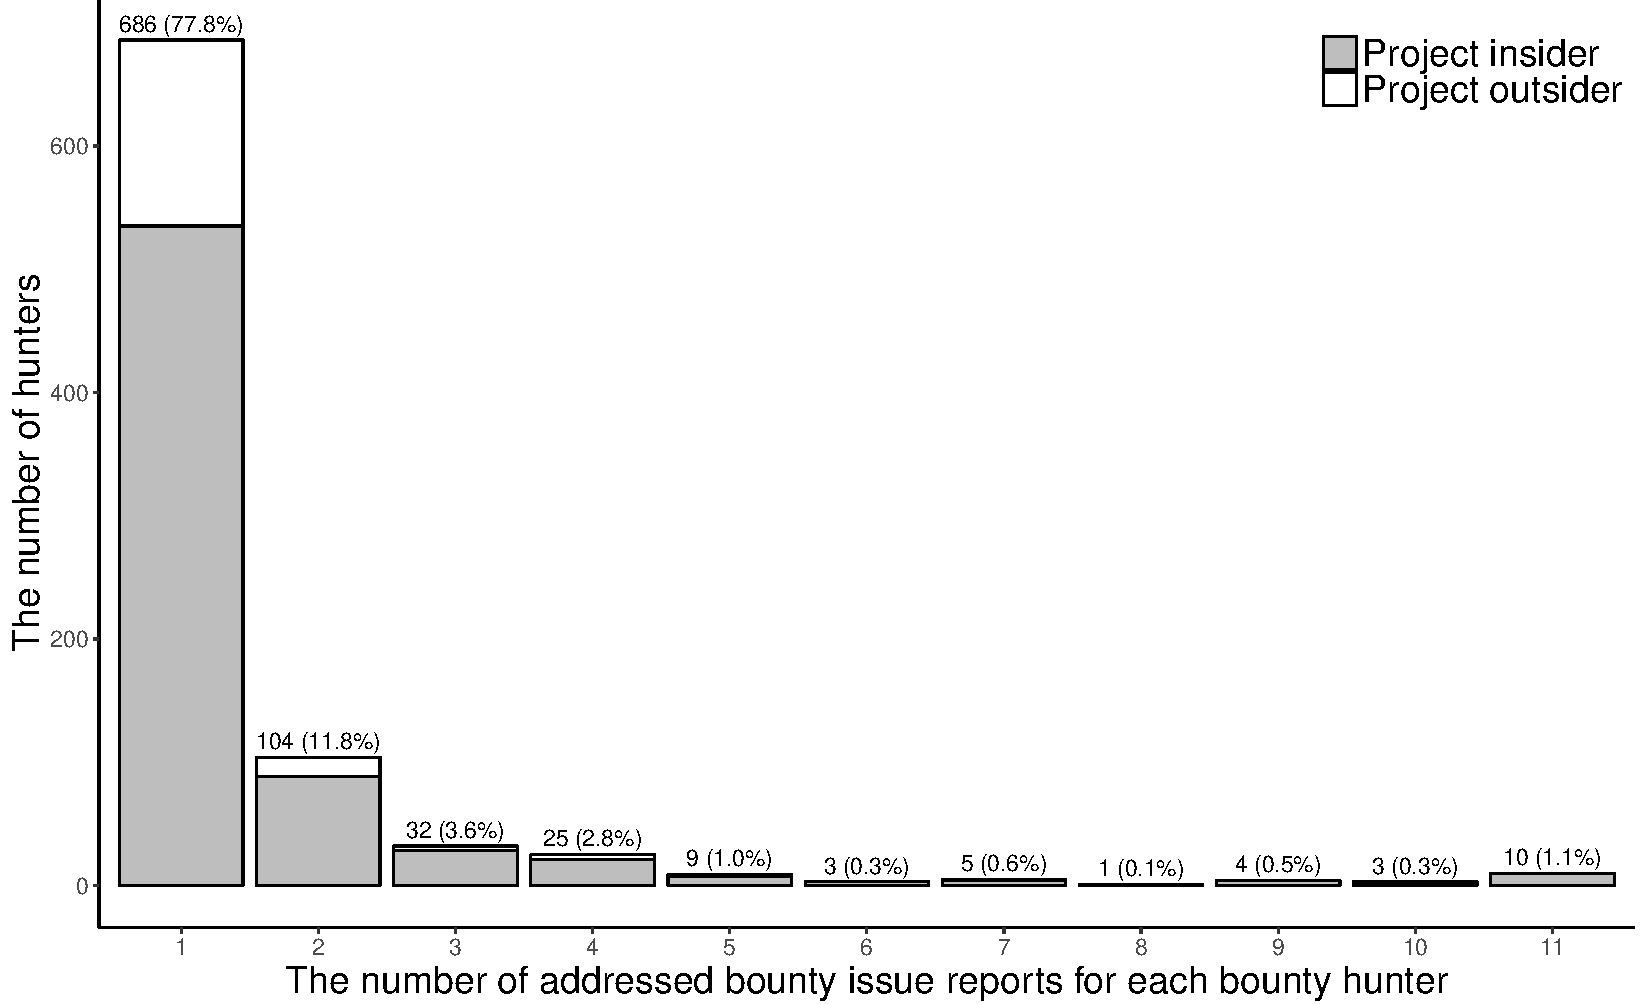
\includegraphics[width=\columnwidth]{pics/rq2/newrq2_distribution_hunter_issue_cnt.pdf}
%  \caption{The number and proportion (presented at the top of each bar) of hunters that addressed x bounty issue reports in the past.  }
%  \label{hunter_isseu_cnt}
%\end{figure}


%479/(479+1508)
\textbf{21.8\% (479 out of 2,200) of the addressed bounty issue reports were not paid out.} We identified that 479 out of the studied 692 bounty issue reports were closed because the issues were addressed. Such cases are interesting since the developers could have claimed the bounty but they did not. We manually examined the discussion for these 479 issue reports. We identified 19 cases in which developers gave an explanation for not claiming the bounty. We grouped the explanations as follows:

\noindent\textbf{The developer is not driven by money.} In 7 out of 19 cases a developer refused to claim the bounty because they were not motivated by money to address the issue.
For example, one developer was against the bounty because they felt that the issue-addressing process should be driven by the interests of the community rather than money. A contributor of the \code{Brython} project,%\footnote{\url{https://brython.info/}}
 refused the bounty because he wanted to keep \code{Brython} free from monetary motivations: ``\textit{What is this `bounty' thing? Needless to say, I refuse that anybody (me included, of course) gets paid for anything related to \code{Brython}.}''\footnote{\url{%https://github.com/brython-dev/brython/issues/680\#issuecomment-330474874
http://bit.ly/2OTYx0x}} In addition, he also asked bounty backers to remove all bounties within the \code{Brython} project although he respected prior bounties that were paid out. There were five bounty issue reports in the \code{Brython} project and four bounty issue reports that were addressed without claiming the bounty.

%Similarly to the \code{Brython} project, the owner of the \code{Pi-hole} project\footnote{\url{https://pi-hole.net/}}, shut down\footnote{\url{https://github.com/pi-hole/pi-hole/issues/371\#issuecomment-379938463}} the usage of the bounty within \code{Pi-hole} because he believed \code{Pi-hole} should be driven by the community need instead of money.
%The developers refused to receive bounties directly since they think that financial incentive should not be involved in open source projects.

\noindent\textbf{The developer is afraid of sending the wrong message.} Krishnamurthy et al. \cite{krishnamurthy2006bounty} pointed out that financial incentives may cause confusion in the community because the financial incentives may drive a project's own product development cycle away from what is in place.
We observed that developers expressed similar concerns. A developer of the \code{Facebook/HHVM} project,%\footnote{\url{https://hhvm.com/}}
 explained that: ``\emph{That's very generous of you, but I can't accept a bounty for doing my job. :-P It would be a conflict of interest, and I worry it sends the wrong message about how we prioritize issues from the community.}''\footnote{\url{%https://github.com/facebook/hhvm/issues/1203\#issuecomment-55794203
http://bit.ly/2OZw1uw}}

%In another example, a developer of the \code{OSVR} project\footnote{\url{http://www.osvr.org/}} refused to claim the bounty and explained: ``\textit{I've already been paid for my part in this code, so I'm happy to see the bounty distributed to the others.}''




\noindent\textbf{The issue report was addressed by more than one developer.} We found nine cases where bounties ended up unclaimed because an issue report was addressed by multiple developers cooperatively and they felt inappropriate to claim the bounty by one developer. For example, the issue\footnote{\url{%https://github.com/numixproject/numix-icon-theme/issues/450/\#issuecomment-143499209
http://bit.ly/2PrMiHV}} was addressed by two developers and because a bounty cannot be split into two parts, no one claimed it.





\subsection{The implications of our findings}
\textbf{Backers should consider proposing a bounty as early as possible and be cautious when proposing small bounties on long-standing issue reports.}
The timing of proposing a bounty is an important factor that impacts the issue-addressing likelihood. In Sections~\ref{rq2} and~\ref{rq3}, we revealed the fact that issue reports for which bounties were proposed earlier are more likely to be addressed. Additionally, we observed that issue reports for which bounties were proposed earlier are more likely to be addressed faster. Backers benefit from the higher issue-addressing likelihood and faster issue-addressing speed by proposing bounties earlier.

In Section~\ref{rq2}, we also noticed a big drop (i.e., from 53.2\% to 30.1\%) of the issue-addressing likelihood when backers proposed bounties on long-standing (i.e., more than half a year) issue reports. This drop might be due to such issue reports having become obsolete or being hard to address.
Since bounties with a value of less than \$100 will not be refunded to the backers if the issue report remains unaddressed, we suggest that backers be cautious when proposing small bounties on long-standing issue reports.

\textbf{Backers should consider proposing a relatively bigger bounty in first-timer bounty-projects.} %In %Section~\ref{rq1}, we observed a positive relationship between the issue-addressing likelihood and the bounty-usage frequency. The global models in Section~\ref{rq3} also show similar results.
Although the issue-addressing likelihood is only 37.4\%  for projects with no bounty-usage experience, the first-timer model in Section~\ref{rq3} shows that the bounty value of an issue report is the most important factor in the first-timer projects, as the issue-addressing likelihood is higher for higher bounty values. The high ratio (2.5) of the bounty value of successful bounty issue reports to the bounty value of failed bounty issue reports also supports this finding.
We suggest that backers of projects with no bounty-usage experience propose higher bounty values for issue reports.


\textbf{Bounty platforms should allow for splittable multi-hunter bounties.}
In addition to a voluntary nature, open source projects have a collaborative nature. Some issues are hard for a developer to address alone. Hence, we encourage developers to work together, especially for issue reports which have a high bounty value (as these issue reports are often harder to address).
However, the current bounty workflow only allows \textbf{one} bounty hunter to claim the bounty, which goes against the collaborative nature of open source. It may also drive the developers, who want to collaboratively address the issue, away because not every participant will get a reward at the end. Therefore, bounty platforms should consider adding the ability for a bounty to be split across multiple hunters to encourage developers to work together on difficult bounty issues.


\textbf{Bounties should be transferable.}
The total value of all addressed-unpaid bounties (\$43,256) is ``frozen'' in Bountysource. In addition, the median number of days between the closing date of the issue report and the date of collecting our data is 372.5,  which means that more than half of the bounties from the ignored bounty issue reports were unclaimed for at least one year. 
By manually examining these 479 addressed-unpaid bounty issue reports, we found 31 cases in which someone reminded the bounty hunter to claim the bounty, however, the reminder was ignored. By reassigning these unclaimed bounties to other issue reports, a larger value could be created for these ``stale'' bounties. For example, Bountysource can suggest and enable backers to assign their long-standing unclaimed bounties to another unaddressed issue report, which has many comments (i.e., people care about it), to encourage developers to address the issue report. Interestingly, we also found suggestions from developers who did not want to receive the bounty but suggested the bounty backers transferring the bounty to other issue reports or to the project as a kind of funding.






\section{Threats to Validity}
\label{sec:threats}
In this section, we discuss the threats to validity.
%\textbf{External validity.}
Threats to \textbf{external validity} are related to the generalizability of our findings. We studied only bounty issue reports from GitHub and Bountysource. Further research is necessary to find whether our findings are generalizable to other types of issue reports (e.g., from commercial platforms) and other bounty platforms.
Although our models have a high explanatory power, there might be additional factors that relate to the likelihood of an issue being addressed. Future studies should investigate more factors.


%\textbf{Internal validity.}
Threats to \textbf{internal validity} relate to the experimenter bias and errors.
One threat relates to the project categorization in Section~\ref{rq1}, in which we used 50 bounty issue reports as a threshold to distinguish whether a project uses bounties moderately or frequently. To alleviate this threat, we redid the analysis of Section~\ref{rq1} with other bounty-usage frequency thresholds (i.e., 40 and 60). %The result shows that the issue-addressing likelihood and the ratio of the bounty value between successful and failed issue reports using different bounty-usage frequency thresholds (see the visualization of the results in Appendix).
The results show that our findings still hold (see our online appendix~\cite{appendix} for more details).


Another threat is that we rely on manual analysis to identify the addressed-unpaid issues and to identify why developers did not claim a bounty in Section~\ref{rq4}, which may introduce bias due to human factors. To mitigate the threat of bias during the manual analysis, two of the authors conducted the manual analysis and discussed conflicts until a consensus was reached. We used Cohen's kappa~\cite{cohenkappa} to measure the inter-rater agreement and the value is 0.86, which indicates a high level of agreement.

%\label{limitation}
%\textbf{External validity.} Threats to external validity relate to the
generalizability of our findings. In this study, we focus on
Stack Overflow, which is one of the most popular Q\&A websites for developers, hence, our results may not generalize
to other Q\&A websites. To alleviate this threat, more Q\&A
websites should be studied in the future.
We needed to conduct several qualitative analysis in
our RQs; however, it is impossible to manually study all
revisions. To minimize the bias when conducting our qualitative analysis, we took statistically representative samples
of all relevant revisions with 95\% confidence level and 5%
confidence interval~\citep{StatisticsInANutshell,conf/msr/ChenSYHGNF16}. 


\emph{Internal validity.} Threats to internal validity relate to experimenter bias and errors. Our study involved qualitative analysis in RQs. To reduce the
bias, each revision was labeled by two of the authors and
discrepancies were discussed until a consensus was reached.
We also showed that the level of inter-rate agreement of the
qualitative studies is high. Another threat of our study is caused by the way we collect the data. The accuracy of our selection criteria is 80\%, which imply that we include the noise in our quantitative study. Future study should develop more accurate method to identify the obsoleteness in Stack Overflow. 

%In addition, the conclusion drawn from our quantitative and qualitative study is based on previous obsolete information we can find on Stack Overflow. In the future the community may have different trends and patterns that we do not expect. However, our conclusion can still be useful for developers to understand better about historical obsolete knowledge on Stack Overflow. 

%=================== Related Work Here =================%
\section{Related work}
\label{relatedwork}
In this section, we discuss related work along two dimensions: the bounty in software engineering and the improvement of the issue-addressing process.

\textit{Bounties in software development:}
Bounties are used to attract developers and motivate them to complete tasks. Prior work has studied the impact of bounties on software development. \cite{krishnamurthy2006bounty} gave an overview of bounties in Free/Libre/Open Source Software (FLOSS).
They observed that bounty hunters' responses are related to the workload, the probability of winning the bounty, the value of the bounty and the recognition that they might receive by winning the bounty. Different from their study, we focused on using bounties to improve the issue addressing process.

\begin{comment}
    Once the profit is higher than the workload, they will respond to the bounty. However, it is very hard to evaluate the profit and workload in an accuracy way.
\end{comment}

Several studies focused on the usage of bounties to motivate developers to detect software security vulnerabilities.
Finifter et al.~\cite{finifter2013empirical} analyzed vulnerability rewards programs for Chrome and Firefox. They found that the rewards programs for both projects are economically effective, compared to the cost of hiring full-time security researchers.
Zhao et al.~\cite{zhao2014exploratory} investigated the characteristics of hunters in bug-bounty programs and found that the diversity of hunters improved the productivity of the vulnerability discovery process. Hata et al.~\cite{hata2017understanding} found that most hunters are not very active (i.e., they have only a few contributions). These findings are similar to our finding that most hunters only addressed one bounty issue. %Hata et al.~\cite{hata2017understanding} performed a user study to understand why developers made a contribution to the bug-bounty program and found that most of the contributors were driven by other factors (e.g., using the product) than money.
Zhao et al. and Maillart et al.~\cite{zhao2017devising,maillart2017given} analyzed the effect of different policies of bug-bounty programs.
By studying bug-bounties from several perspectives, they provided insights on how to improve the bug-bounty programs. For example, Maillart et al.~\cite{maillart2017given} suggested project managers to dynamically adjust the value of rewards according to the market situation (e.g., increase rewards when releasing a new version).
%They found bounty programs more cost-effective compared to hiring full-time security researchers in terms of finding security flaws


However, there is not much research to study the effectiveness of bounties in the issue-addressing process.
The work of Kanda et al.~\cite{kanda2017towards} is closest to ours. They studied GitHub and Bountysource data but studied only 31 projects (compared to 1,203 in our study). They compared the closed-rate and closing-time between bounty issue and non-bounty issue reports. Their results showed that the closing-rate of bounty issue reports is lower than that of non-bounty issue reports, and it takes longer for the bounty issue reports to get closed than non-bounty issue reports.
%They also analyzed the top three bounty backers and found that some big-value bounties were provided to directly hire developers rather than reward bounty hunters.
Our study performs a deeper analysis of bounties at the project and the time level. Besides, we further study the relationship between the issue-addressing likelihood and the bounty-related factors (e.g., the total bounty value of a bounty issue report) while controlling for the factors that are related to the issue report and project (e.g., the number of comments before the first bounty is proposed). We found that the timing and the bounty-usage frequency are the most important factors in increasing the issue-addressing likelihood.


\textit{Improving the issue-addressing process:}
%Developers and users are encouraged to report issues in issue tracking systems because the feedback from user communities is important for the evolution of a software development project (\cite{bagozzi2006open,hendry2008public}). %\cite{bissyande2013got} further investigated the popularity and impact of issue trackers and revealed the relation between issue reporters and issues.
Issue addressing is an essential activity in the life cycle of software development and maintenance. Therefore, a large amount of research was done to improve the issue-addressing process.
One group of studies focused on providing insights into improving the issue-addressing process in aspects of the quality of issue reports, the effectiveness of developers and automated bug localization and fixing.
For example, Bettenburg et al.~\cite{bettenburg2008makes,hooimeijer2007modeling} analyzed the quality of bug reports (i.e., a type of issue report) and provided some guidelines for users to generate high-quality reports so that developers can address issues more efficiently. Ortu et al.~\cite{Ortu:2015} analyzed the relation between sentiment, emotions, and politeness of developers in comments with needed time to address an issue. They found that the happier developers are, the shorter the issue-addressing time is likely to be. Zhong et al.~\cite{Zhong:2015} performed an empirical study on real-world bug fixes to provide insights and guideline for improving the state-of-the-art of automated program repair. Soto et al.~\cite{Soto:2016} performed a large-scale study of bug-fixing commits in Java projects and provided insights for high-quality automated software repair to target Java code.
A number of studies helped developers locate the buggy code in projects using information retrieval techniques~\cite{Zhou:2012,Saha:2013,WangL16,WangLL14}.
\begin{comment}

Another group of studies focused on developing automated tools to facilitate the issue-addressing process. \cite{Zhou:2012,Saha:2013,WangL16,WangLL14} leveraged textual and structural information in a bug report to help developers locate the buggy code in projects using information retrieval techniques. \cite{Lam:2015,XiaoKMB17} leveraged deep learning techniques to facilitate the bug localization task.
\cite{anvik2006should} invented an SVM-based approach to semi-automatically assign bug reports to developers. \cite{hosseini2012market} improved bug assignment mechanism with a market-based approach to speed up the bug-fixing process. \cite{XuanJHRZLW15,hu2014effective,goyal2017effective} proposed an approach to recommend suitable developers to fix bugs.

\end{comment}
Different from prior studies, we perform an empirical study to understand the relationship between bounties and the issue-addressing process. We provide insights into how to better use the bounty to improve the issue-addressing process.




%=================== Conclusion Here =================%
\section{Conclusion}
\label{conclusion}


In this paper, we studied 5,445 bounties with a total value of \$406,425 from Bountysource along with their associated 3,509 issue reports from GitHub to study the relationship between the bounty (e.g., timing of proposing a bounty, bounty value, and bounty-usage frequency) and the issue-addressing likelihood.
We found that:
\begin{enumerate}
\item The timing of proposing bounties and the bounty-usage frequency are the most important factors that impact the issue-addressing likelihood. Issue reports for which bounties were proposed earlier are more likely to have a higher issue-addressing likelihood and a faster addressing-speed. 
\item In first-timer bounty-projects, the issue-addressing likelihood is higher for higher bounty values and in these projects, backers should consider proposing a relatively bigger bounty. 
\item Backers should be cautious when proposing small bounties on long-standing issue reports as they risk losing money without getting their issue addressed.
\end{enumerate}


Our findings suggest that backers should consider proposing a bounty early and be cautious when proposing small bounties on long-standing issue reports. Bounty platforms should allow dividing bounties between hunters, and transferring bounties to other issue reports.






%=================== References Here =================%
\balance
\bibliographystyle{abbrv}
{
\footnotesize
\bibliography{ref}
}

\begin{comment}
\begin{IEEEbiography}[{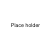
\includegraphics[width=1in,height=1.25in,clip,keepaspectratio]{bio/jiayuan.png}}]{Jiayuan Zhou}
Jiayuan Zhou
\end{IEEEbiography}

% if you will not have a photo at all:
\begin{IEEEbiography}[{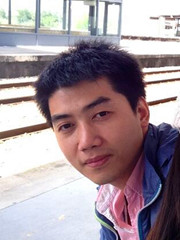
\includegraphics[width=1in,height=1.25in,clip,keepaspectratio]{bio/shaowei.jpg}}]{Shaowei Wang}
Shaowei Wang
\end{IEEEbiography}

% insert where needed to balance the two columns on the last page with
% biographies
%\newpage

\begin{IEEEbiography}[{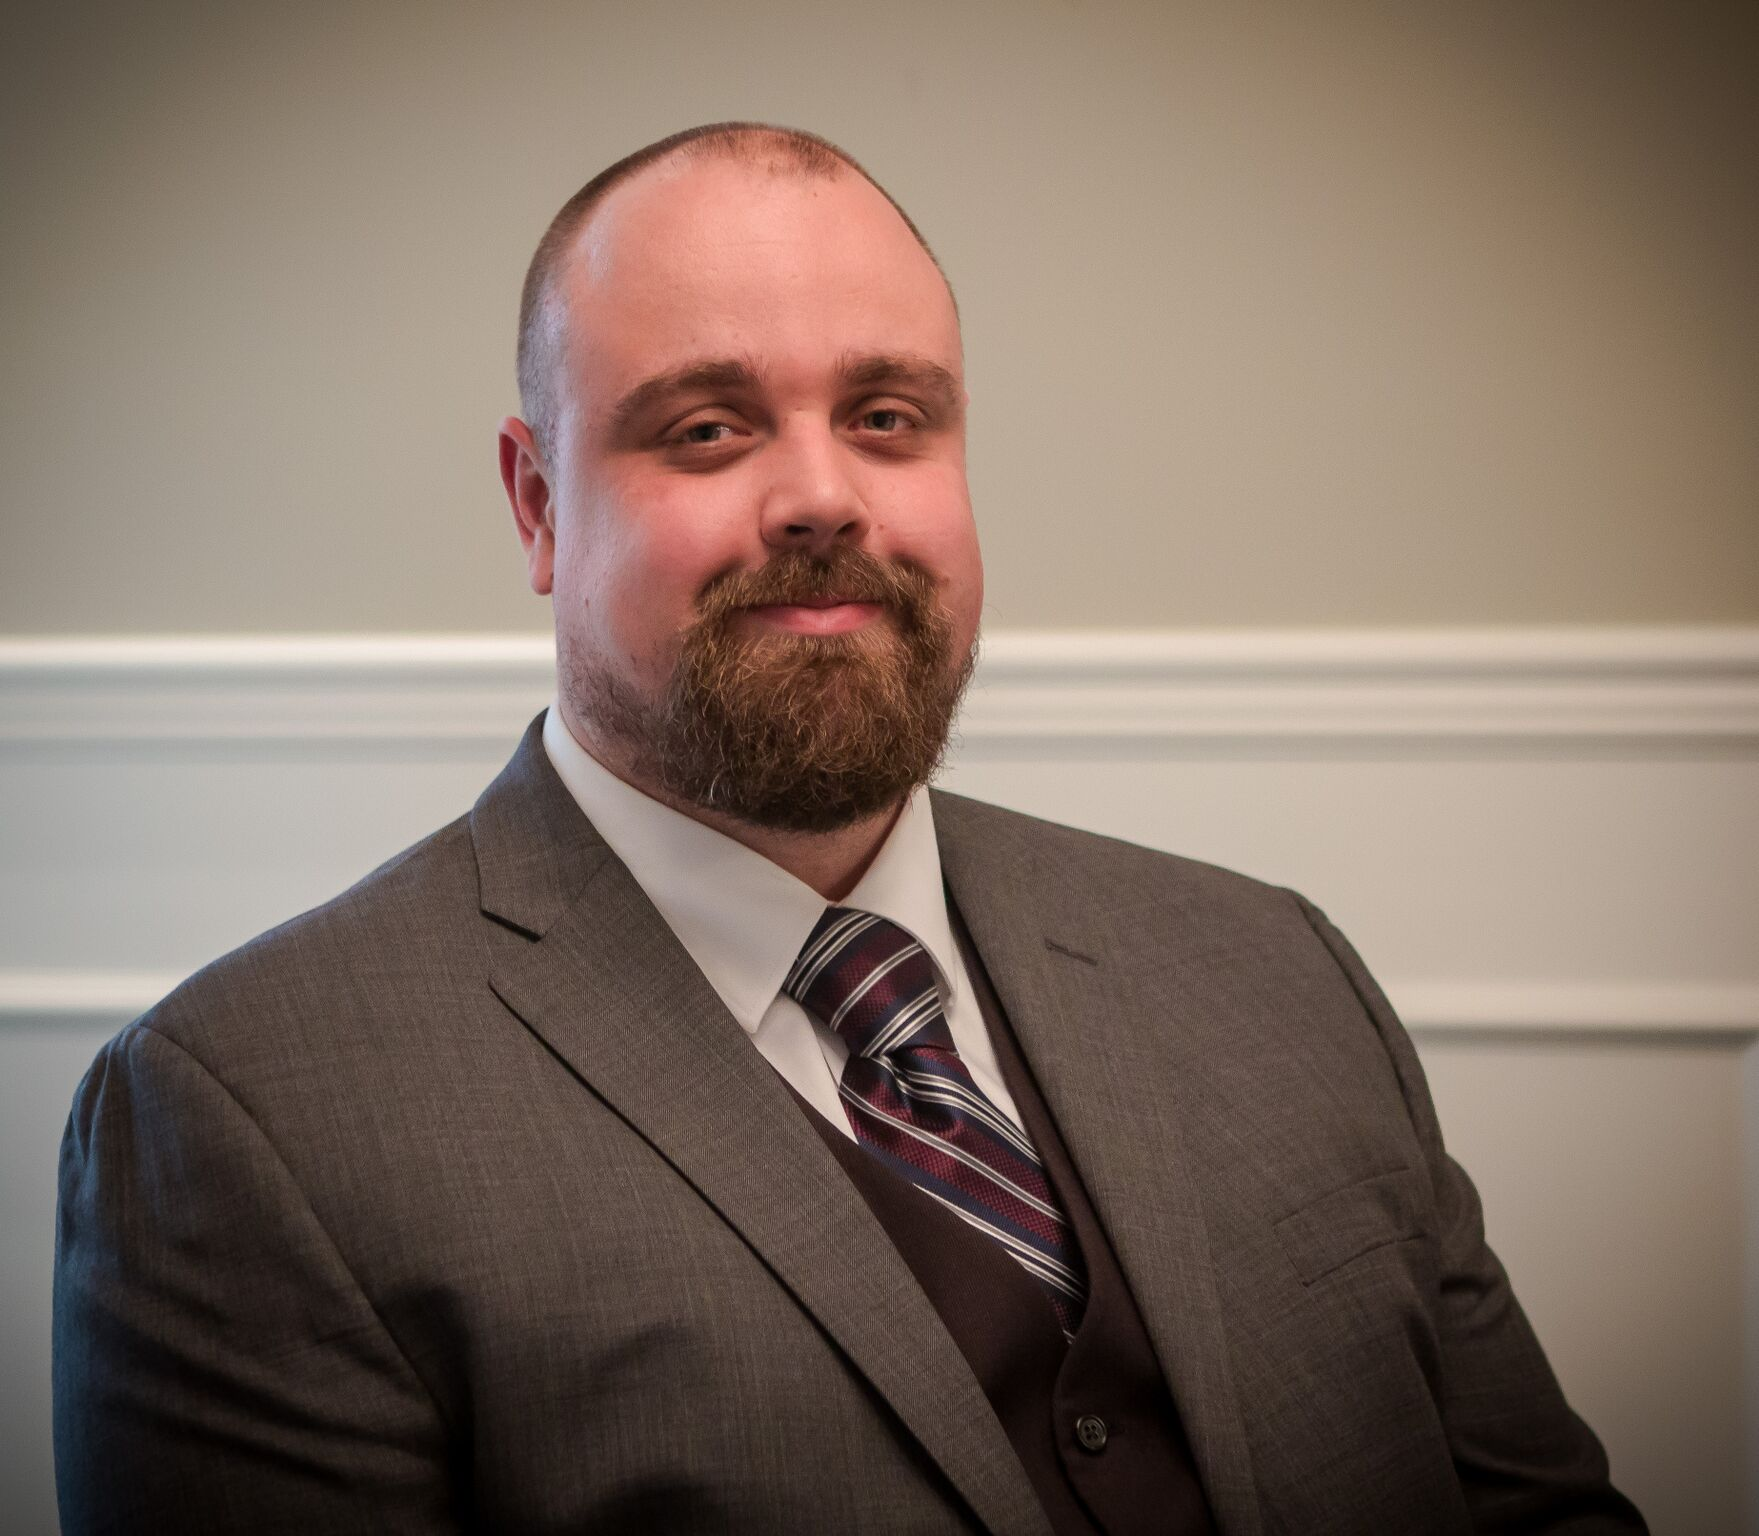
\includegraphics[width=1in,height=1.25in,clip,keepaspectratio]{bio/corpaul.png}}]{Cor-Paul~Bezemer}
Cor-Paul~Bezemer
\end{IEEEbiography}

\begin{IEEEbiography}[{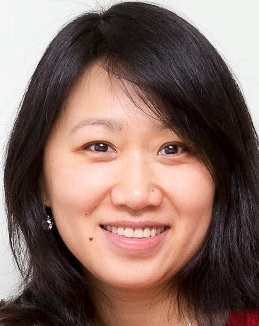
\includegraphics[width=1in,height=1.25in,clip,keepaspectratio]{bio/jenny.jpg}}]{Ying Zou}
Ying Zou
\end{IEEEbiography}

\begin{IEEEbiography}[{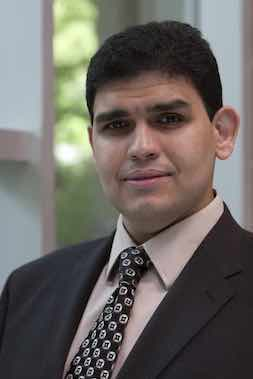
\includegraphics[width=1in,height=1.25in,clip,keepaspectratio]{bio/ahmed.png}}]{Ahmed E. Hassan}
Ahmed E. Hassan
\end{IEEEbiography}
\end{comment}

%\begin{appendices}
%\renewcommand \appendixname{Appendix}
%\label{appendix}
%\RequirePackage{fix-cm}
\documentclass[10pt,journal,compsoc]{IEEEtran}
\usepackage{cite}
\usepackage{graphicx}
\usepackage{multirow}
\usepackage{hhline}
\usepackage{comment}
\usepackage[dvipsnames]{xcolor}
\usepackage[colorlinks=false, linkcolor=blue, citecolor=blue, bookmarks=true,pagebackref=false]{hyperref}
\usepackage{subcaption}
\usepackage{float}
\usepackage{caption}
\usepackage{fancybox}
\usepackage{array,booktabs}
\usepackage{marvosym} % For the \Letter command
%\usepackage{textcomp} % arrow
%\usepackage{tablefootnote} % footnote in table
\usepackage{balance}
\usepackage{ragged2e}
\usepackage{makecell}
\usepackage{bigstrut}
%\usepackage[title]{appendix}

\begin{document}
	\begin{appendices}
%=================== Model construction =================%
	This appendix will be available online~\cite{appendix}. We included it as supplementary material for the convenience of the anonymous reviewers.

      \section{Model construction}
      In this section, we elaborate on the details of our model construction process. Figure~\ref{fig:flowMC} shows an overview of our model construction process. The process can be broken down into following three steps:
	
	  \begin{figure}[b]
        \centering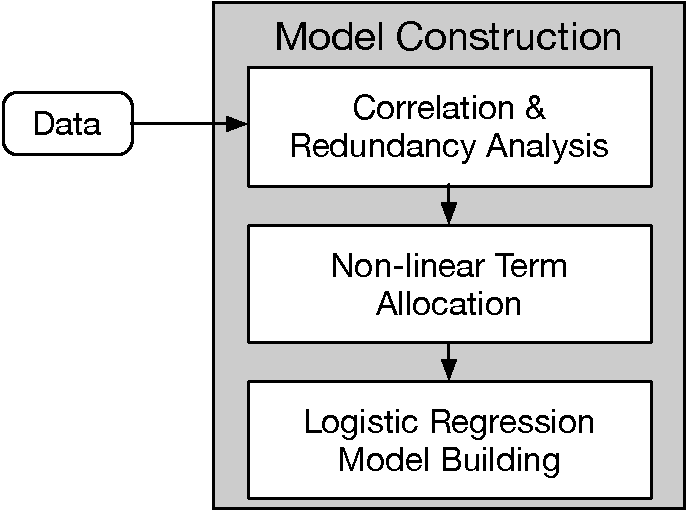
\includegraphics[width=.7\columnwidth]{pics/appendix/mondelconstruction}
        \caption{The overview our model construction process.}
        \label{fig:flowMC}
        \vspace{-0.2in}
      \end{figure}
	
	\begin{enumerate}
		\item \textbf{Correlation \& Redundancy Analysis:}  Similar to prior studies~\cite{gopi:2017,wang2017understanding,mcintosh2016empirical,kabinna2018examining}, we remove correlated and redundant factors to avoid multicollinearity.
      First, we use the Spearman rank correlation test to measure the correlation between factors and remove highly-correlated factors (using a cut-off value of 0.7 \cite{gopi:2017,wang2017understanding,mcintosh2016empirical,kabinna2018examining}). For each of the highly-correlated factors, we keep one factor in the model. Figure~\ref{FINAL_RQ3_hie} shows the results of our correlation analysis, and the factors that were eventually used in the models. Then we apply a redundancy analysis and remove redundant factors.
      Finally, we end up with three factors in the project bounty dimension, six factors in the issue report basic dimension, four factors in the issue report bounty dimension, and three factors in the backer experience dimension.
      Because factors which have a constant value do not contribute explanatory power to a logistic regression model, we remove factors which are constant within a project group when building the corresponding models. For example, we remove \textit{P\_B\_usage\_group} (i.e., bounty-usage frequency) for the first-timer models , the moderate models and the frequent models since \textit{P\_B\_usage\_group} is a constant value for these models. In addition, we remove all project bounty-related factors for the first-timer bounty-projects since for these projects the values of all project bounty-related factors are 0.

	
      \begin{figure}[t]
        \centering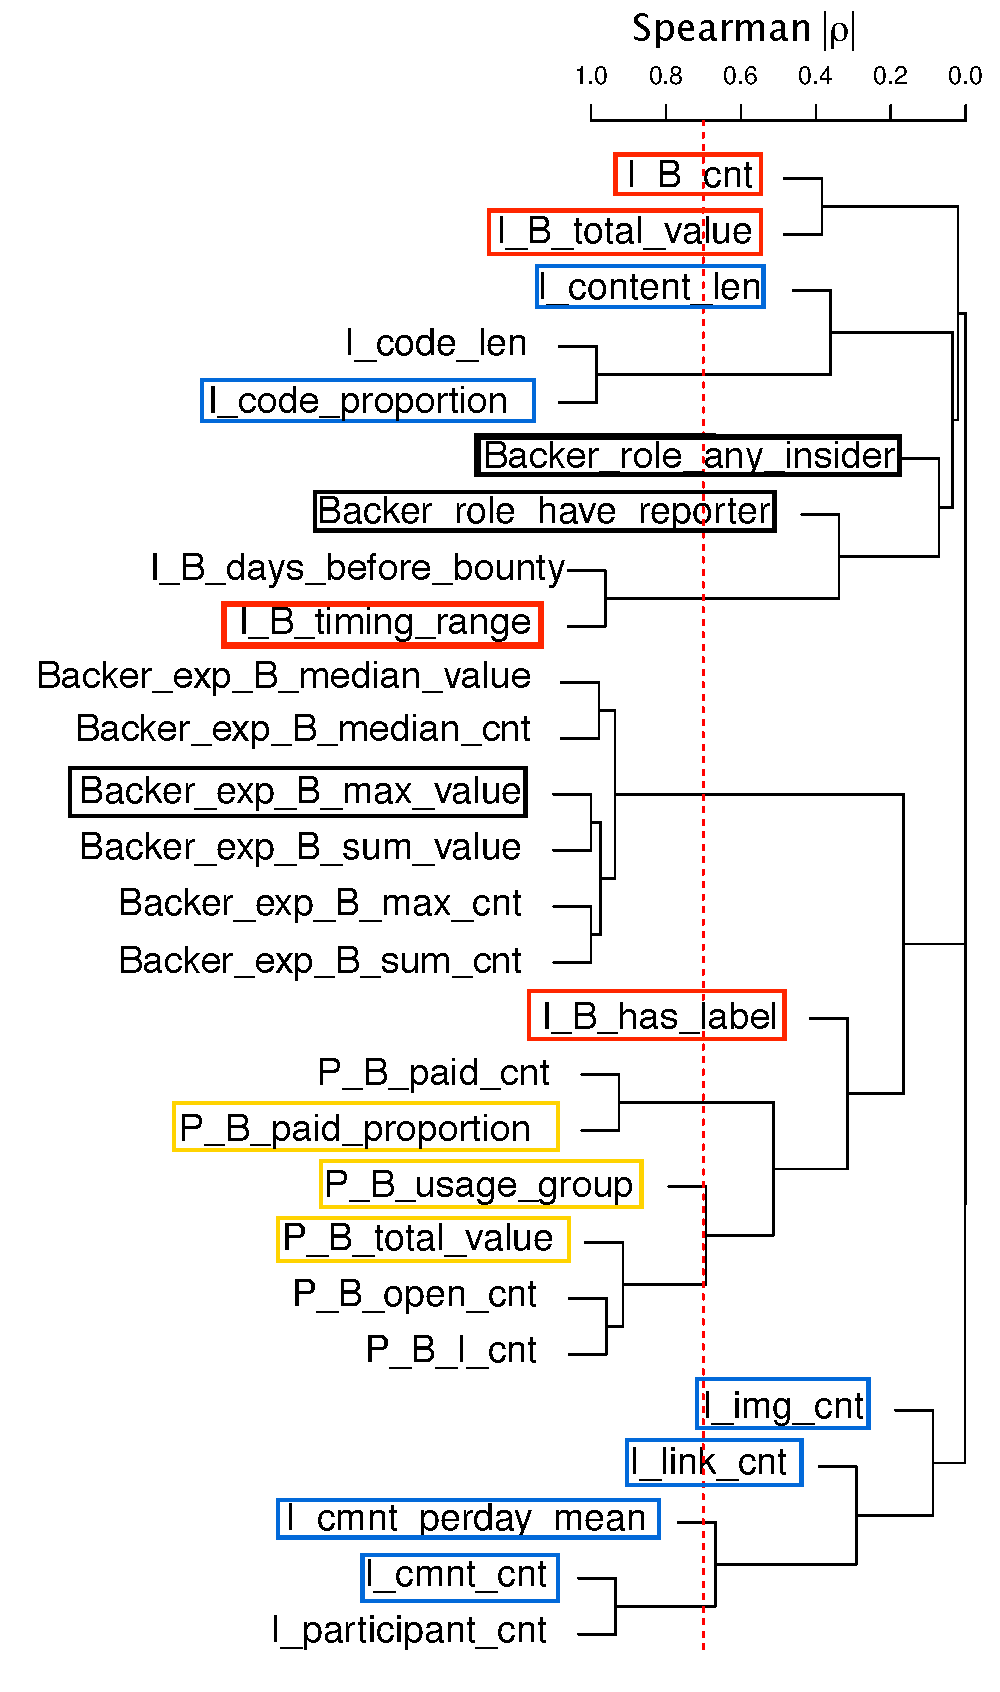
\includegraphics[width=\columnwidth ]{pics/rq3/rq3_hie}
        \caption{The hierarchical clustering plot of factors according to the Spearman rank correlation test (using a cut-off value of 0.7). We selected the simplest metrics to compute across each dimension of correlated factors. We ended up with three factors in the project level dimension (marked in yellow), six factors in the issue report basic dimension (marked in blue), four factors in the issue report bounty dimension  (marked in red), and three in the backer-related factors dimension (marked in black).}
        \label{FINAL_RQ3_hie}
        \vspace{-0.2in}
      \end{figure}
      \begin{figure}[h]
        \centering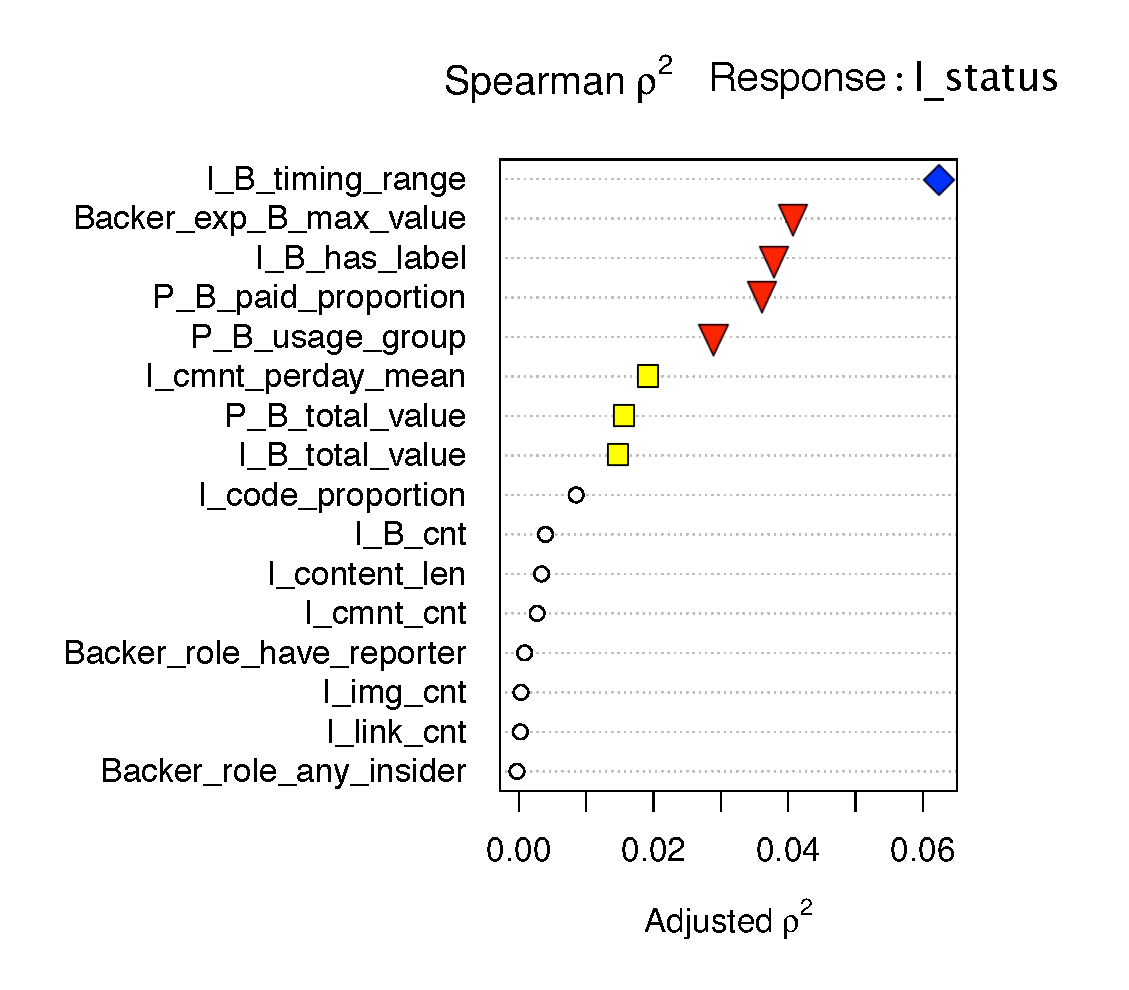
\includegraphics[width=\columnwidth]{pics/rq3/rq3_spearman}
        \caption{Dotplot of the Spearman multiple ${\rho}^2$  of each factor in all the bounty issue reports. The larger the ${\rho}^2$ value, the more likely the factor has a non-linear relationship with the response variable. By observing the rough clustering of the factors according to their $\rho^2$, we cluster the factors into four groups according
        to the Spearman multiple $\rho^2$  values. We assign the first, second, and third groups of factors (categorized by the ${\rho}^2$ value) which are highlighted with a blue diamond, red triangle, and yellow square, 5, 4, and 3 degrees of freedom, respectively.  }
        \label{fig:rq3_spearman}
      \end{figure}

    \item \textbf{Non-linear Term Allocation:}
      Similar to prior work~\cite{mcintosh2016empirical, wang2017understanding}, we add non-linear terms (i.e., NL) in each model to capture the more complex relationship in the data by employing restricted cubic splines~\cite{Harrell:2006}. The non-linear factor will be assigned more degrees of freedom (i.e., D.F.). We calculated the Spearman multiple $\rho^2$ between the dependent factor and each explanatory factor to measure their non-linear relationship. If a factor has a higher $\rho^2$, it indicates that it has a higher chance of having a non-linear relationship with the dependent factor. We therefore assigned this factor more degrees of freedom.
      Figure~\ref{fig:rq3_spearman} shows the Spearman multiple $\rho^2$ of the studied factors. By observing the rough clustering of the
      factors according to their $\rho^2$, we cluster the factors into four groups according to the Spearman multiple $\rho^2$  values. The factor marked by the blue diamond is assigned five degrees, factors marked by red triangles are assigned four degrees and factors marked by yellow squares are assigned three degrees of freedom.
      We use the R package \textbf{rms}\footnote{\url{https://cran.r-project.org/web/packages/rms/index.html}} to implement our logistic regression model.

      \item \textbf{Logistic Regression Model Building:} Finally, we built four groups of logistic regression models (i.e., the first-timer, moderate, frequent, and global models) based on 100 samples and ended up with 400 models.


	\end{enumerate}
	
	
	
%=================== Model analysis =================%

      \section{Model analysis}
      In this section, we elaborate on the details of our model analysis process. The process includes two parts:
      \begin{enumerate}
      	\item \textbf{Model Assessment:}  For a logistic regression model, we use the Area Under the Receiver Operating Characteristic Curve (i.e., AUC) and a bootstrap-derived approach \cite{efron1986biased} to assess the explanatory power of the models following prior studies~\cite{mcintosh2016empirical,wang2017understanding,kabinna2018examining}. The AUC ranges from 0 to 1 (0.5 is the performance of a random guessing model) and a higher AUC means that the model has a higher ability to capture the relationships between the explanatory factors and the response factor.

     		 For each sample, we use a bootstrap-derived approach~\cite{efron1986biased} to validate the performance of models. We first build a model with a bootstrapped sample and calculate the AUC (i.e., the \textit{bootstrapped\_AUC}). Then we apply the model to the original sample and calculate the AUC (i.e., the \textit{original\_AUC}). After that, we use the optimism value, which is the difference between the \textit{bootstrapped\_AUC} and \textit{original\_AUC} to evaluate the degree of overfitting of the model. A small optimism value indicates that the model does not suffer from overfitting.
    		  We repeated the bootstrap-derived approach for 100 iterations for each sample and used the median \textit{bootstrapped\_AUC} and the median optimism value to represent the performance of models for that sample.
    		  Finally, we built 10,000 (100 samples * 100 bootstrap-derived iterations) models for each group of models.
     		 For each group of models, we use the median optimism value and the median AUC of all samples to evaluate the stability of the models. In order to condense our writing, we use the \textit{median AUC} and the \textit{median optimism value} to express the above concepts.
     		 
         \item \textbf{Explanatory Variables Analysis:}   
			We further study the impact of each factor on the issue-addressing likelihood by using the \textbf{anova} function in the R \textbf{rms} package to compute the Wald $\chi^2$ value.
  		    The larger the Wald $\chi^2$ value of a factor is, the larger impact of the factor on the issue-addressing likelihood.
   			For each sample, we computed the Wald $\chi^2$ value for each factor. Then we use the median Wald $\chi^2$ value of each factor to represent the impact of that factor.

    		In addition, to further understand how a factor influences the value of the response variables, we use the \textbf{Predict} function in the \textbf{rms} R package to plot the estimated issue-addressing likelihood against a factor. %Since all models across 100 samples showed similar patterns of influence for the factors, we randomly selected a sample as an example to build models and visualize the results (see Figure~\ref{fig:rq3_trend}).
      		%The analysis allows us to further understand how a factor affects the issue-addressing likelihood. %We hold the other factors at their median values when exploring a specific factor.
      \end{enumerate}
      Table~\ref{tab:rq3_analysis} shows the results of our model analysis. 

   
       % Table generated by Excel2LaTeX from sheet 'Sheet2'
       \begin{table*}[]
      % \tiny
         \centering
         \caption{The results of the model analysis for four groups of models. We highlight the most important variable of models of each group in bold. The \textbf{NL} indicates the non-linear term and the \textbf{D.F.} indicates the degree of freedom.}
           \begin{tabular}{lp{0.5cm}p{0.8cm}rp{0.9cm}rp{0.8cm}rp{0.8cm}r}
           \toprule
           \multicolumn{2}{p{1.7cm}}{} & \multicolumn{2}{p{8em}}{\textbf{Global Models}} & \multicolumn{2}{p{1.7cm}}{\textbf{First-timer Model}s} & \multicolumn{2}{p{1.7cm}}{\textbf{Moderate Models}} & \multicolumn{2}{p{1.7cm}}{\textbf{Frequent Models}} \bigstrut[b]\\
           \midrule
           \multicolumn{2}{p{8em}}{Median AUC} & \multicolumn{2}{l}{0.72} & \multicolumn{2}{l}{0.74} & \multicolumn{2}{l}{0.71} & \multicolumn{2}{l}{0.81} \bigstrut[t]\\
           \multicolumn{2}{p{15em}}{Median Optimism Value} & \multicolumn{2}{l}{0.02} & \multicolumn{2}{l}{0.03} & \multicolumn{2}{l}{0.04} & \multicolumn{2}{l}{0.03} \bigstrut[b]\\
           \midrule
           \multicolumn{2}{l}{Factors} & Overall & \multicolumn{1}{p{3em}}{NL} & Overall & \multicolumn{1}{p{3em}}{NL} & Overall & \multicolumn{1}{p{3em}}{NL} & Overall & \multicolumn{1}{p{3em}}{NL} \bigstrut\\
           \midrule
           \multicolumn{1}{l}{\multirow{2}[2]{*}{I\_B\_timing\_range}} & D.F.  & 1     &       & 1     &       & 1     &       & 1     &  \bigstrut[t]\\
                 & $\chi^2$ & \textbf{47.87***} &       &6.68* &       & \textbf{18.12***} &       & \textbf{21.26***} &  \bigstrut[b]\\
           \midrule
           \multicolumn{1}{l}{\multirow{2}[2]{*}{P\_B\_usage\_group}} & D.F.  & 1     &       & -     &       & -     &       & -     &  \bigstrut[t]\\
                 & $\chi^2$ & \textbf{28.38***} &       & -     &       & -     &       & -     &  \bigstrut[b]\\
           \midrule
           \multicolumn{1}{l}{\multirow{2}[2]{*}{I\_B\_total\_value}} & D.F.  & 2     & \multicolumn{1}{p{4em}}{1} & 2     & \multicolumn{1}{p{3em}}{1} & 2     & \multicolumn{1}{p{3em}}{1} & 2     & \multicolumn{1}{p{5.085em}}{1} \bigstrut[t]\\
                 & $\chi^2$ & 9.58** & \multicolumn{1}{p{4em}}{7.21**} & \textbf{23.06***} & \multicolumn{1}{p{3em}}{0.13} & 2.0   & \multicolumn{1}{p{3em}}{0.31} & 6.57* & \multicolumn{1}{p{5.085em}}{4.81*} \bigstrut[b]\\
           \midrule
           \multicolumn{1}{l}{\multirow{2}[2]{*}{I\_code\_proportion}} & D.F.  & 1     &       & 1     &       & 1     &       & 1     &  \bigstrut[t]\\
                 & $\chi^2$ & 10.97** &       & 1.97  &       & 6.20* &       & 1.96  &  \bigstrut[b]\\
           \midrule
           \multicolumn{1}{l}{\multirow{2}[2]{*}{I\_B\_has\_label}} & D.F.  & 1     &       & 1     &       & 1     &       & 1     &  \bigstrut[t]\\
                 & $\chi^2$ & 14.75*** &       & 4.40* &       & 3.41  &       & 0.93  &  \bigstrut[b]\\
           \midrule
           \multicolumn{1}{l}{\multirow{2}[2]{*}{Backer\_exp\_B\_max\_value}} & D.F.  & 3     & \multicolumn{1}{p{4em}}{2} & 3     & \multicolumn{1}{p{3em}}{2} & 3     & \multicolumn{1}{p{3em}}{2} & 3     & \multicolumn{1}{p{5.085em}}{2} \bigstrut[t]\\
                 & $\chi^2$ & 9.14* & \multicolumn{1}{p{4em}}{7.88*} & 1.39  & \multicolumn{1}{p{3em}}{0.23} & 2.13  & \multicolumn{1}{p{3em}}{0.67} & 13.55** & \multicolumn{1}{p{5.085em}}{12.87**} \bigstrut[b]\\
           \midrule
           \multicolumn{1}{l}{\multirow{2}[2]{*}{P\_B\_paid\_proportion}} & D.F.  & 3     & \multicolumn{1}{p{4em}}{2} & -     &       & 3     & \multicolumn{1}{p{3em}}{2} & 3     & \multicolumn{1}{p{5.085em}}{2} \bigstrut[t]\\
                 & $\chi^2$ & 11.22* & \multicolumn{1}{p{4em}}{4.98} & -     &       & 4.23  & \multicolumn{1}{p{3em}}{0.58} & 16.43** & \multicolumn{1}{p{5.085em}}{15.37***} \bigstrut[b]\\
           \midrule
           \multicolumn{1}{l}{\multirow{2}[2]{*}{P\_B\_total\_value}} & D.F.  & 2     & \multicolumn{1}{p{4em}}{1} & -     &       & 2     & \multicolumn{1}{p{3em}}{1} & 2     & \multicolumn{1}{p{5.085em}}{1} \bigstrut[t]\\
                 & $\chi^2$ & 9.85** & \multicolumn{1}{p{4em}}{8.96**} & -     &       & 1.40  & \multicolumn{1}{p{3em}}{0.10} & 15.42*** & \multicolumn{1}{p{5.085em}}{13.46***} \bigstrut[b]\\
           \midrule
           \multicolumn{1}{l}{\multirow{2}[2]{*}{I\_img\_cnt}} & D.F.  & 1     &       & 1     &       & 1     &       & 1     &  \bigstrut[t]\\
                 & $\chi^2$ & 1.62  &       & 1.25  &       & 0.79  &       & 1.28  &  \bigstrut[b]\\
           \midrule
           \multicolumn{1}{l}{\multirow{2}[2]{*}{I\_link\_cnt}} & D.F.  & 1     &       & 1     &       & 1     &       & 1     &  \bigstrut[t]\\
                 & $\chi^2$ & 0.41  &       & 0.48  &       & 0.55  &       & 0.91  &  \bigstrut[b]\\
           \midrule
           \multicolumn{1}{l}{\multirow{2}[2]{*}{I\_content\_len}} & D.F.  & 1     &       & 1     &       & 1     &       & 1     &  \bigstrut[t]\\
                 & $\chi^2$ & 1.76  &       & 0.29  &       & 0.84  &       & 1.97  &  \bigstrut[b]\\
           \midrule
           \multicolumn{1}{l}{\multirow{2}[2]{*}{I\_cmnt\_perday\_mean}} & D.F.  & 2     & \multicolumn{1}{p{4em}}{1} & 2     & \multicolumn{1}{p{3em}}{1} & 2     & \multicolumn{1}{p{3em}}{1} & 2     & \multicolumn{1}{p{5.085em}}{} \bigstrut[t]\\
                 & $\chi^2$ & 7.60* & \multicolumn{1}{p{4em}}{2.52} & 4.42  & \multicolumn{1}{p{3em}}{0.15} & 1.32  & \multicolumn{1}{p{3em}}{0.58} & 1.28  & \multicolumn{1}{p{5.085em}}{} \bigstrut[b]\\
           \midrule
           \multicolumn{1}{l}{\multirow{2}[2]{*}{I\_B\_cnt}} & D.F.  & 1     &       & 1     &       & 1     &       & 1     &  \bigstrut[t]\\
                 & $\chi^2$ & 0.80  &       & 0.94  &       & 1.12  &       & 7.76** &  \bigstrut[b]\\
           \midrule
           \multicolumn{1}{l}{\multirow{2}[2]{*}{I\_cmnt\_cnt}} & D.F.  & 1     &       & 1     &       & 1     &       & 1     &  \bigstrut[t]\\
                 & $\chi^2$ & 0.35  &       & 1.72  &       & 0.30  &       & 2.10  &  \bigstrut[b]\\
           \midrule
           \multicolumn{1}{l}{\multirow{2}[2]{*}{Backer\_role\_any\_insider}} & D.F.  & 1     &       & 1     &       & 1     &       & 1     &  \bigstrut[t]\\
                 & $\chi^2$ & 1.78  &       & 5.81* &       & 0.32  &       & 0.67  &  \bigstrut[b]\\
           \midrule
           \multicolumn{1}{l}{\multirow{2}[1]{*}{Backer\_role\_have\_reporter}} & D.F.  & 1     &       & 1     &       & 1     &       & 1     &  \bigstrut[t]\\
                 & $\chi^2$ & 0.52  &       & 0.45  &       & 0.69  &       & 0.38  &  \\
                 \bottomrule
      \multicolumn{10}{l}{P-value of the $\chi^2$ test: `***' $<$ 0.001; `**' $<$ 0.01; `*' $<$ 0.05} \bigstrut[t]\\
           \end{tabular}%
         \label{tab:rq3_analysis}%
       \end{table*}%


      \section{Additional result for threats to validity}

      \begin{figure*}[th]
        \centering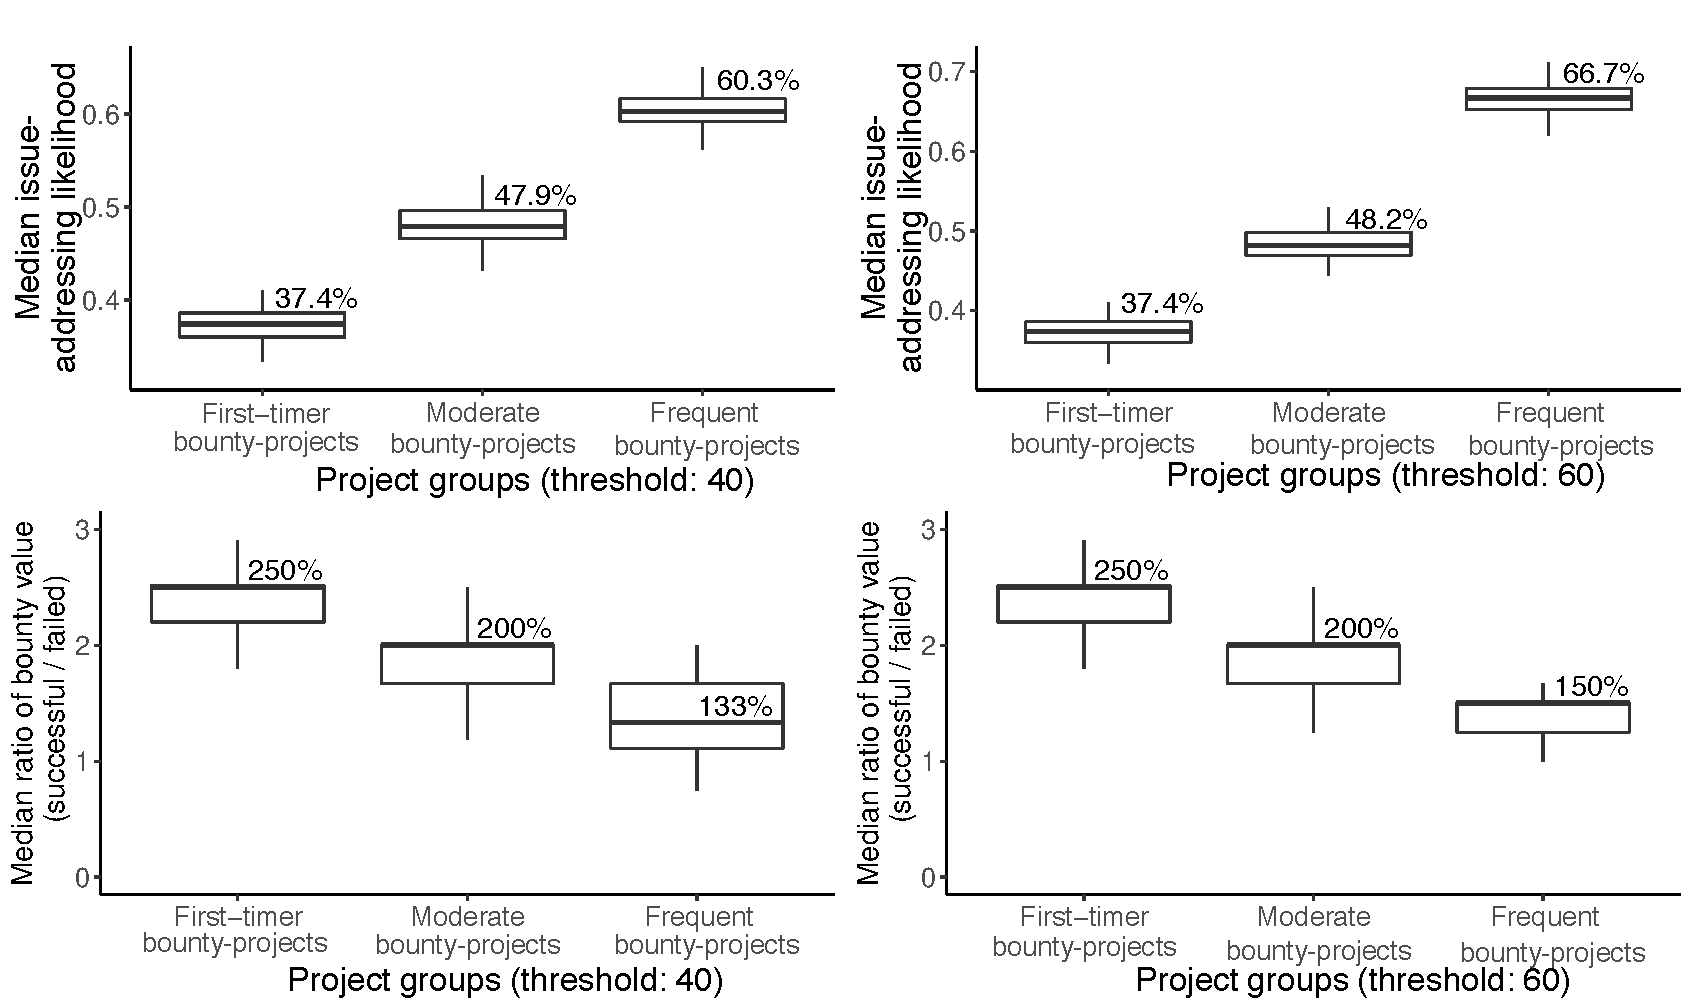
\includegraphics[width=\textwidth ]{pics/threat/threat}
        \caption{The distribution of the median issue-addressing likelihood and the median ratio of bounty value when using different thresholds for the separation across different project groups.}
        \label{fig:threat}
      \end{figure*}
      In this section, we visualize the result of our analysis in the threats to validity section regarding different bounty-usage frequency thresholds. Figure~\ref{fig:threat} shows  the distribution of the median issue-addressing likelihood and the median ratio of bounty value when using different thresholds for the separation across different project groups. Figure~\ref{fig:threat} shows that our results are not affected by our choice for the threshold for the bounty-usage frequency.

      \balance
      \bibliographystyle{abbrv}
      {
      \footnotesize
      \bibliography{ref}
      }
  \end{appendices}
\end{document}

%\end{appendices}



\end{document}
